\documentclass[12pt,a4paper]{article}
\usepackage[left=4cm,right=3cm,top=3cm,bottom=3cm]{geometry}
\usepackage{mathptmx} % Times New Roman
\usepackage[T1]{fontenc}
\usepackage{textcomp}
\usepackage{amsmath}
\usepackage{amssymb}
\usepackage{graphicx}
\usepackage{float}
\usepackage{hyperref}
\usepackage[none]{hyphenat}
\usepackage{tikz}
\usepackage{enumitem}
\usepackage{titlesec}
\usepackage{multirow}
\usepackage{setspace}
\usepackage{ragged2e}
\usepackage{caption}

% Pengaturan hyphenation untuk Bahasa Indonesia
\sloppy % Membuat LaTeX lebih fleksibel dengan spacing
\tolerance=9999
\emergencystretch=3em
\hbadness=9999
\hyphenpenalty=10000
\exhyphenpenalty=50
\doublehyphendemerits=10000
\finalhyphendemerits=5000
\pretolerance=100

% Pengaturan paragraf: tanpa indentasi dan jarak minimal antar paragraf
\setlength{\parindent}{0pt} % Menghilangkan indentasi awal paragraf
\setlength{\parskip}{0pt} % Tidak ada jarak antar paragraf

% Pengaturan jarak untuk subsection
\titleformat{\subsection}{\normalsize\bfseries}{\thesubsection}{1em}{}
\titlespacing*{\subsection}{0pt}{0pt}{0pt} % Tidak ada jarak sebelum atau setelah judul

% Pengaturan jarak untuk subparagraph
\titleformat{\subparagraph}[runin]{\normalsize\bfseries}{\thesubparagraph}{1em}{}
\titlespacing*{\subparagraph}{0pt}{0pt}{1em} % Memberikan sedikit spasi setelah judul

% Pengaturan spasi
\onehalfspacing

% Pengaturan penomoran
\renewcommand{\thesection}{\Roman{section}}
\renewcommand{\thesubsection}{\thesection.\arabic{subsection}}
\renewcommand{\thesubsubsection}{\thesubsection.\arabic{subsubsection}}
\renewcommand{\thesubparagraph}{\thesubsubsection.\arabic{subparagraph}}

% Pengaturan label dan caption
\renewcommand{\figurename}{Gambar}
\renewcommand{\tablename}{Tabel}
\captionsetup[figure]{justification=centering}
\captionsetup[table]{justification=centering}

\begin{document}

\sloppy

\vspace{2cm}
\begin{center}
{\fontsize{14}{16.8}\selectfont\textbf{BAB III. Metodologi Penelitian}}\\[1em]
\end{center}
\label{sec:metodologi}
\addcontentsline{toc}{section}{BAB III METODOLOGI PENELITIAN}
\setcounter{section}{3}
\setcounter{subsection}{0}
\vspace{2em}

Bab ini menguraikan pendekatan penelitian yang mengintegrasikan \textit{Design Science Research Methodology} (DSRM) sebagai kerangka sistematis untuk identifikasi masalah, penetapan tujuan, desain, evaluasi, dan komunikasi hasil penelitian. Metodologi ini dipilih karena kesesuaiannya dengan tujuan penelitian, yaitu merancang, mengembangkan, dan mengevaluasi sebuah artefak berupa \textit{framework} restorasi dokumen berbasis GAN dengan Diskriminator Dual-Modal dan fungsi \textit{loss} berorientasi HTR. Implementasi teknis \textit{framework} dilakukan melalui siklus iteratif \textit{deep learning} yang berbasis bukti empiris dan dokumentasi sistematis.
\vspace{1em}

\subsection{Kerangka Teori Metodologi Penelitian}
\label{subsec:kerangka-teori}
\vspace{0.8em}

\subsubsection{\textit{Design Science Research Methodology} (DSRM)}

\begin{figure}[htbp]
\centering
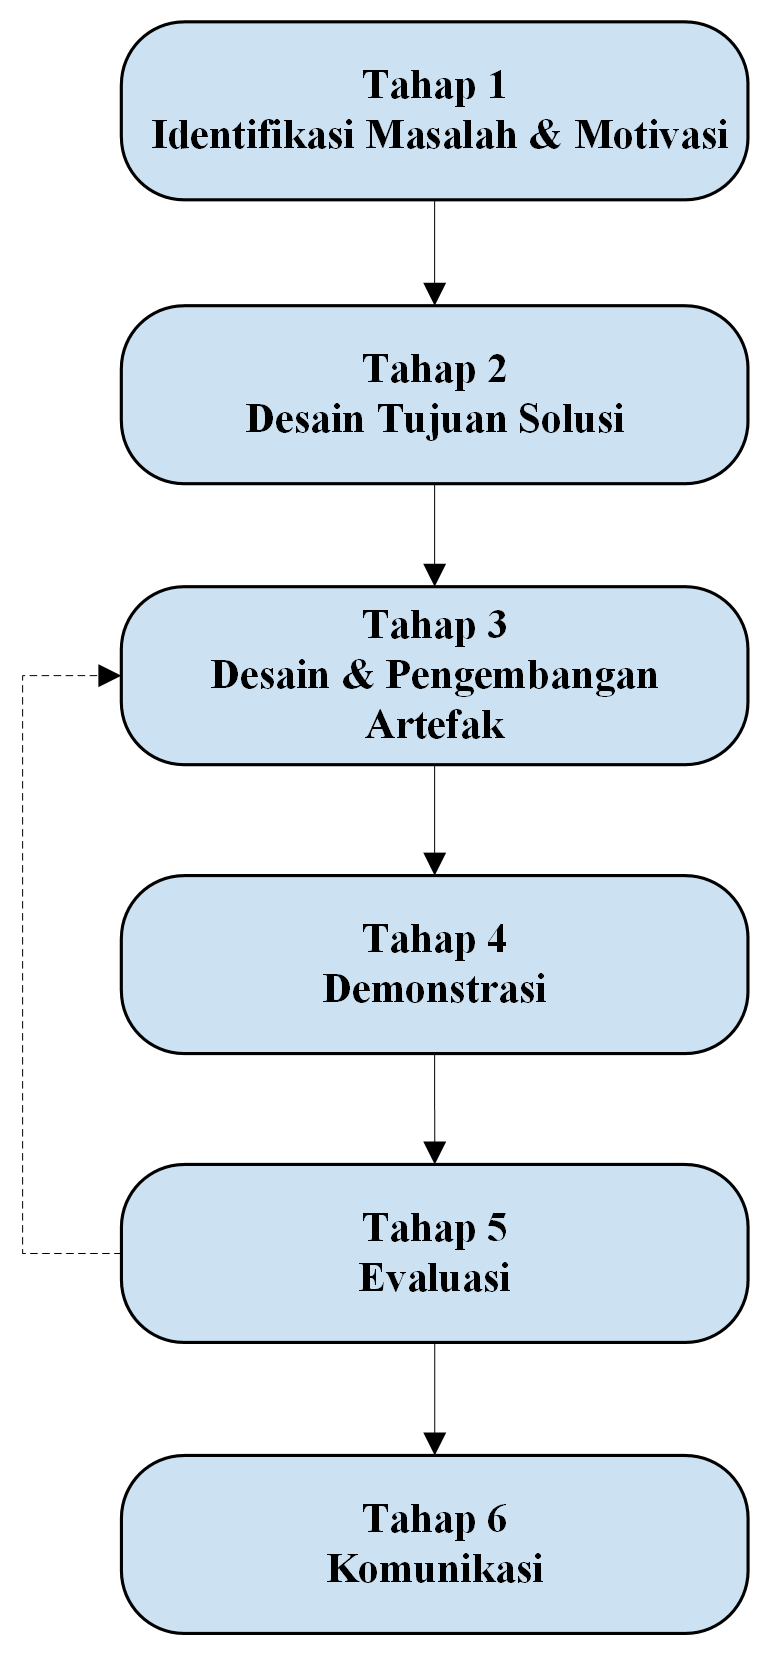
\includegraphics[width=0.3\textwidth]{images/DRSM.png}
\caption{Framework Design Science Research Methodology yang diadaptasi untuk penelitian ini dengan siklus iteratif antara evaluasi dan desain untuk penyempurnaan artefak.}
\label{fig:dsrm-framework}
\end{figure}

\textit{Design Science Research Methodology} (DSRM), yang diperkenalkan oleh Peffers et al. (2007), merupakan kerangka penelitian yang dirancang khusus untuk pengembangan dan evaluasi artefak teknologi informasi. DSRM terdiri dari enam tahapan yang saling terkait dan bersifat iteratif, di mana hasil dari tahap evaluasi memberikan umpan balik untuk penyempurnaan pada tahap desain dan pengembangan.

\subsubsection{Adaptasi DSRM untuk Pengembangan \textit{Framework} GAN-HTR}
Karakteristik utama DSRM yang relevan dengan penelitian ini adalah:

\begin{enumerate}[label=\arabic*., leftmargin=*, nosep]
\item \textbf{Orientasi Solusi:} DSRM berfokus pada penciptaan artefak inovatif untuk menyelesaikan masalah praktis yang teridentifikasi. Dalam konteks penelitian ini, artefak yang dikembangkan adalah \textit{framework} GAN dengan Diskriminator Dual-Modal yang secara eksplisit dioptimalkan untuk meningkatkan keterbacaan dokumen oleh sistem HTR.

\item \textbf{Evaluasi Berbasis Bukti:} Setiap iterasi desain dievaluasi secara kuantitatif menggunakan metrik yang terukur (PSNR, SSIM, CER, WER), memastikan bahwa penyempurnaan dilakukan berdasarkan data empiris bukan asumsi.

\item \textbf{Siklus Iteratif:} Kerangka kerja ini memfasilitasi perbaikan berkelanjutan melalui putaran umpan balik (\textit{feedback loop}) antara tahap evaluasi dan desain, yang sangat sesuai dengan karakteristik pengembangan model \textit{deep learning} yang memerlukan eksperimen dan \textit{tuning} berulang.

\item \textbf{Komunikasi dan Diseminasi:} DSRM menekankan pentingnya mendokumentasikan dan mengkomunikasikan hasil penelitian kepada komunitas ilmiah, baik melalui publikasi akademis maupun berbagi kode sumber untuk reproduktifitas.
\end{enumerate}

\subsubsection{Siklus Iteratif Berbasis Bukti Empiris}
Penelitian ini mengadopsi siklus iteratif yang berbasis bukti empiris untuk memastikan setiap keputusan desain didukung oleh data yang valid. Setiap tahap evaluasi menghasilkan temuan kuantitatif yang menjadi dasar untuk penyempurnaan artefak pada iterasi berikutnya. Pendekatan ini meminimalkan subjektivitas dan meningkatkan validitas ilmiah dari hasil penelitian.

\subsection{Tahapan Penelitian}
\label{subsec:tahapan-penelitian}

Penelitian ini mengikuti enam tahapan DSRM yang telah diadaptasi untuk konteks pengembangan \textit{framework} restorasi dokumen berbasis \textit{deep learning}. Setiap tahapan dijelaskan secara rinci berikut dengan metode, perangkat lunak, dan dokumentasi yang digunakan.

\subsubsection{Identifikasi Masalah dan Motivasi (Tahap 1)}
Tahap pertama berfokus pada analisis mendalam terhadap tantangan yang ada dalam restorasi dokumen historis dan identifikasi kesenjangan penelitian yang menjadi motivasi pengembangan framework baru.

\paragraph{Aktivitas Utama:}

\begin{enumerate}[label=\arabic*., leftmargin=*, nosep]
\item \textbf{Studi Literatur Sistematis}

Dilakukan kajian komprehensif terhadap penelitian terkait restorasi dokumen, GAN, dan HTR untuk mengidentifikasi keterbatasan metode yang ada. Fokus utama pada analisis metode \textit{state-of-the-art} seperti DE-GAN, TEXT-DIAE, dan CycleGAN.

\item \textbf{Analisis Kebutuhan Praktis}

Dilakukan analisis terhadap kebutuhan nyata lembaga kearsipan, dalam hal ini Arsip Nasional Republik Indonesia, di mana restorasi digital harus mendukung transkripsi otomatis untuk aksesibilitas dan analisis data historis. Identifikasi menunjukkan bahwa dokumen kolonial Belanda mengalami degradasi kompleks: \textit{bleed-through}, \textit{fading} tinta \textit{iron gall}, noda air (\textit{water stains}), bercak kecokelatan (\textit{foxing}), dan kabur optik (\textit{optical blur}) dari proses pemindaian.

\item \textbf{Perumusan Masalah Penelitian}

Berdasarkan analisis literatur dan kebutuhan praktis, dirumuskan masalah utama penelitian: ``Bagaimana merancang arsitektur GAN yang secara eksplisit dioptimalkan untuk meningkatkan keterbacaan teks oleh sistem HTR, bukan hanya kualitas visual, pada dokumen historis dengan degradasi kompleks?''

Masalah ini diformulasikan menjadi empat pertanyaan penelitian yang telah dijelaskan pada Bab I.
\end{enumerate}

\subsubsection{Definisi Tujuan Solusi (Tahap 2)}
Berdasarkan masalah yang teridentifikasi, tujuan dari artefak yang akan dibangun didefinisikan secara kuantitatif dan kualitatif dengan target yang terukur.

\paragraph{Tujuan Kuantitatif:}

Penelitian ini menetapkan target performa yang dapat diukur dan diverifikasi:

\begin{table}[H]
\centering
\caption{Target metrik kuantitatif penelitian}
\label{tab:target-metrik}
\small
\begin{tabular}{|l|l|l|}
\hline
\textbf{Kategori} & \textbf{Metrik} & \textbf{Target} \\ \hline
\multirow{2}{*}{Kualitas Visual} & PSNR & $>$ 35 dB \\ \cline{2-3}
 & SSIM & $>$ 0.95 \\ \hline
\multirow{2}{*}{Keterbacaan Teks} & CER & Penurunan signifikan vs baseline \\ \cline{2-3}
 & WER & Penurunan signifikan vs baseline \\ \hline
\multirow{2}{*}{Stabilitas Training} & Generator Loss & Konvergen tanpa mode collapse \\ \cline{2-3}
 & Diskriminator Accuracy & 60-80\% (Nash equilibrium) \\ \hline
Efisiensi Komputasi & Inference Time & $<$ 15 detik per image (1024$\times$128) \\ \hline
\end{tabular}
\end{table}

\paragraph{Tujuan Kualitatif:}

Mendefinisikan fitur inovatif dan kontribusi penelitian:

\begin{enumerate}[leftmargin=*, nosep]
\item \textbf{Diskriminator Dual-Modal:} Merancang arsitektur diskriminator yang mampu mengevaluasi kualitas gambar dari dua perspektif simultan: realisme visual (\textit{visual realism}) dan koherensi teks (\textit{text coherence}).

\item \textbf{Fungsi Loss Berorientasi HTR:} Mengintegrasikan sinyal loss dari model HTR secara langsung ke dalam fungsi loss Generator, menciptakan optimasi ganda.

\item \textbf{Filosofi \textit{Recognizer} Terbekukan:} Menggunakan \textit{recognizer} dengan bobot yang dibekukan sebagai evaluator objektif dengan kualitas metrik yang stabil.

\item \textbf{\textit{Pipeline} Degradasi Sintetis:} Mengembangkan \textit{pipeline} degradasi sintetis yang realistis untuk menghasilkan pasangan pelatihan (\textit{training pairs}) dari dokumen bersih.
\end{enumerate}

\subsubsection{Desain dan Pengembangan Artefak (Tahap 3)}
Tahap ini merupakan inti penelitian di mana artefak (framework GAN-HTR) dirancang, diimplementasikan, dan disempurnakan melalui siklus iteratif berbasis eksperimen. Tahap ini mengikuti metodologi pengembangan deep learning yang terdokumentasi dan mencakup tiga aspek fundamental: penyiapan lingkungan komputasi, manajemen data dan eksperimen, serta pengembangan framework modular.

\begin{figure}[htbp]
\centering
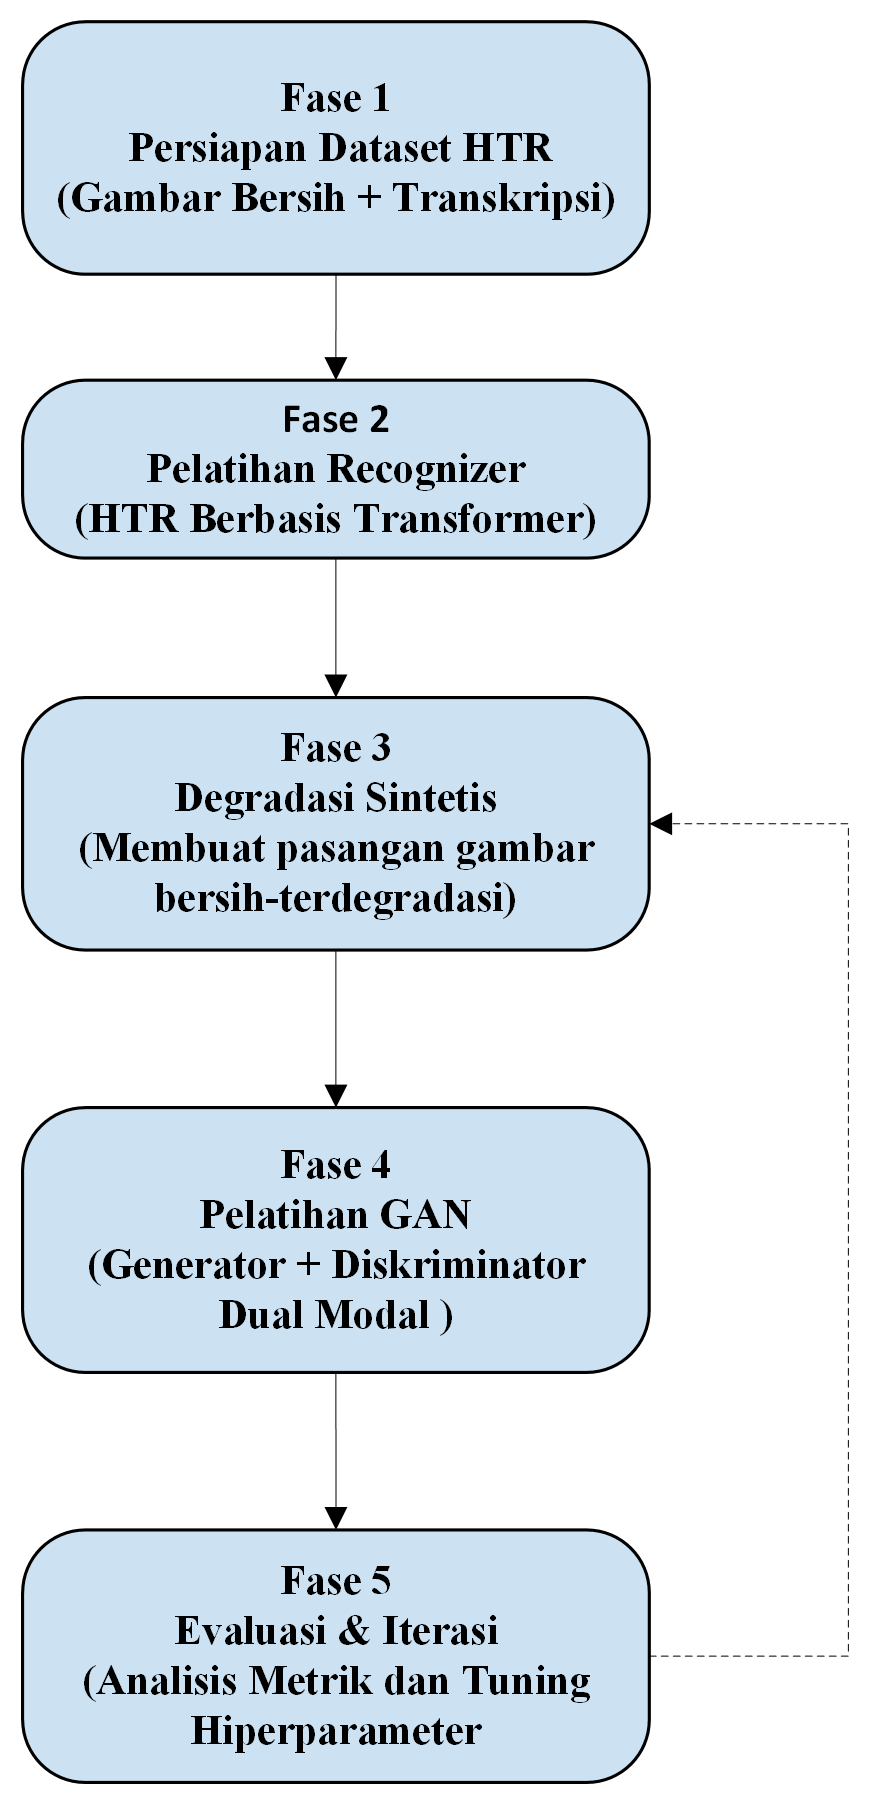
\includegraphics[width=0.35\textwidth]{images/PengembanganArtefak.png}
\caption{\textit{Pipeline} pengembangan \textit{framework} GAN-HTR dengan lima fase utama yang dilakukan secara sekuensial dengan iterasi pada fase 4 dan 5.}
\label{fig:development-pipeline}
\end{figure}

\paragraph{Fase 1: Persiapan Dataset HTR}
Dataset bersih disiapkan untuk melatih model Recognizer dengan struktur yang meliputi input gambar line text bersih, label ground truth transcription, format TFRecord untuk efisiensi loading, dan preprocessing berupa normalisasi intensitas, padding, resizing.

\paragraph{Fase 2: Pelatihan dan Pembekuan Recognizer}
Model Recognizer dilatih menggunakan arsitektur hybrid CNN-Transformer untuk HTR (spesifikasi arsitektur lengkap pada Bab IV bagian 4.2.3 dan Lampiran A). Fase ini mengadopsi metodologi \textit{curriculum learning} dengan tiga strategi kunci untuk mencapai performa optimal dan stabilitas training:

\textbf{Curriculum Learning Strategy}: Penelitian ini menerapkan pendekatan bertahap dalam training Recognizer dimana model pertama-tama difokuskan pada pembelajaran fundamental melalui fase \textit{warmup} (5 epochs awal) dengan learning rate yang meningkat secara linear, kemudian dilanjutkan dengan fase pembelajaran utama menggunakan \textit{cosine annealing schedule}. Pendekatan ini memastikan model tidak terjebak pada local minima di awal training dan mencapai konvergensi yang lebih baik. Rationale: Transformer-based models sangat sensitif terhadap inisialisasi learning rate; warmup mencegah gradient explosion pada early iterations.

\textbf{Data Augmentation untuk Robustness}: Training menggunakan augmentasi data secara real-time pada setiap batch untuk meningkatkan kemampuan generalisasi model terhadap variasi dokumen real-world. Augmentasi mencakup variasi photometric (brightness, contrast) dan noise injection yang mensimulasikan kondisi scanning dan digitalisasi dokumen historis yang beragam. Rationale: Dataset synthetic memiliki distribusi terbatas; augmentasi memperluas ruang input dan mencegah overfitting pada karakteristik synthetic tertentu.

\textbf{Multi-Layer Regularization}: Kombinasi teknik regularisasi diterapkan pada berbagai tingkat arsitektur (dropout pada layers, label smoothing pada loss function, weight decay pada optimizer) untuk mencegah overfitting sambil mempertahankan kapasitas pembelajaran model. Early stopping dengan monitoring validation CER memastikan model berhenti training pada titik optimal sebelum terjadi degradasi performa. Rationale: Sequence-to-sequence models prone to overfitting; multi-layer regularization provides defense-in-depth.

\textbf{Pembekuan Model (Freezing) dan Dual-Purpose Utilization}: Setelah training mencapai convergence (ditandai dengan validation CER stabil), bobot model recognizer dibekukan (\texttt{training=False}) untuk memastikan konsistensi evaluasi selama training GAN. Keputusan freezing ini krusial karena: (1) menjaga stabilitas metrik HTR sebagai ground truth objektif, (2) mencegah \textit{catastrophic forgetting} saat recognizer diekspos ke degraded images, dan (3) memungkinkan reproduktifitas eksperimen dengan evaluator yang konsisten.

Model frozen ini kemudian dimanfaatkan untuk dua tujuan dalam framework GAN-HTR: (1) ekstraksi \textit{recognition features} dari layer intermediate (\texttt{proj\_ln}) untuk \textit{recognition feature loss} yang mengoptimalkan Generator di feature space, dan (2) perhitungan CTC loss yang di-backpropagate ke Generator untuk optimasi keterbacaan langsung di sequence space. Dual-purpose ini merupakan inovasi metodologis yang memungkinkan pembelajaran multi-level dari model HTR frozen.

Detail hyperparameter training, arsitektur layer-by-layer, dan konfigurasi optimizer tersedia pada Lampiran A dan B untuk keperluan reproduksi.

\begin{table}[H]
\centering
\caption{Ringkasan konfigurasi training Recognizer HTR}
\label{tab:recognizer-training-summary}
\small
\begin{tabular}{|l|p{10cm}|}
\hline
\textbf{Komponen} & \textbf{Ringkasan Konfigurasi} \\
\hline
Arsitektur & Hybrid CNN-Transformer (detail: Bab IV.4.2.3, Lampiran A) \\
\hline
Optimizer & AdamW dengan weight decay dan gradient clipping \\
\hline
Learning Rate Schedule & Warmup (5 epochs) + Cosine annealing \\
\hline
Batch Size & 32 \\
\hline
Regularization & Dropout, label smoothing, early stopping (patience=15) \\
\hline
Data Augmentation & Photometric (brightness, contrast) + Noise injection \\
\hline
Precision & FP32 untuk stabilitas numerik CTC \\
\hline
Target Performance & CER $<$ 15\% (achieved $\sim$33\% baseline), WER $<$ 25\% \\
\hline
\multicolumn{2}{|l|}{\\textit{Catatan: Spesifikasi lengkap hyperparameter pada Lampiran B, Tabel \\ref{tab:appendix-optimizer}}} \\
\hline
\end{tabular}
\end{table}

\begin{algorithm}[H]
\caption{Training Procedure: HTR Recognizer}
\label{alg:recognizer-training}
\small
\begin{algorithmic}[1]
\STATE \textbf{Input:} Dataset HTR $\mathcal{D} = \{(x_i, t_i)\}_{i=1}^N$ dengan $x_i$ = image, $t_i$ = transcription
\STATE \textbf{Output:} Trained \& Frozen Recognizer $R_{\theta}$
\STATE \textbf{Hyperparameters:} LR = 3×10$^{-4}$, batch\_size = 32, warmup\_epochs = 5
\STATE
\STATE Initialize CNN-Transformer model $R_{\theta}$ dengan random weights
\STATE Initialize optimizer AdamW dengan weight decay = 2×10$^{-4}$
\STATE
\FOR{epoch = 1 to max\_epochs}
    \STATE // Warmup Phase (epoch 1-5): Linear LR ramp-up
    \IF{epoch $\leq$ warmup\_epochs}
        \STATE $\text{LR}_{\text{current}} = \text{LR}_{\text{max}} \times \frac{\text{epoch}}{\text{warmup\_epochs}}$
    \ELSE
        \STATE // Cosine Annealing: decay LR smoothly
        \STATE $\text{LR}_{\text{current}} = \text{LR}_{\text{min}} + \frac{1}{2}(\text{LR}_{\text{max}} - \text{LR}_{\text{min}})(1 + \cos(\pi \frac{\text{epoch} - \text{warmup}}{\text{total\_epochs}}))$
    \ENDIF
    \STATE
    \FOR{each batch $(X, T)$ in $\mathcal{D}_{\text{train}}$}
        \STATE // Apply real-time augmentation
        \STATE $X_{\text{aug}} \gets$ RandomBrightness(X, $\pm$20\%) + RandomContrast(X, 0.8-1.2) + GaussianNoise(X, $\sigma$=0.08)
        \STATE
        \STATE // Forward pass
        \STATE $\hat{Y} \gets R_{\theta}(X_{\text{aug}})$ \quad // Output: (batch, timesteps, charset+1)
        \STATE
        \STATE // CTC Loss with label smoothing
        \STATE $\mathcal{L}_{\text{CTC}} \gets \text{CTCLoss}(\hat{Y}, T, \epsilon=0.1)$
        \STATE
        \STATE // Backward pass with gradient clipping
        \STATE Compute gradients $\nabla_{\theta} \mathcal{L}_{\text{CTC}}$
        \STATE Clip gradients to norm = 1.0
        \STATE Update $\theta$ using AdamW
    \ENDFOR
    \STATE
    \STATE // Validation
    \STATE Compute $\text{CER}_{\text{val}}$, $\text{WER}_{\text{val}}$ on $\mathcal{D}_{\text{val}}$
    \IF{$\text{CER}_{\text{val}}$ improved}
        \STATE Save checkpoint $R_{\theta}^{\text{best}}$
        \STATE Reset patience counter
    \ELSE
        \STATE Increment patience counter
    \ENDIF
    \IF{patience $\geq$ 15}
        \STATE \textbf{break} \quad // Early stopping
    \ENDIF
\ENDFOR
\STATE
\STATE // Freeze model for GAN training
\STATE Load best checkpoint $R_{\theta}^{\text{best}}$
\STATE Set $R_{\theta}$.trainable = False \quad // Freeze all weights
\STATE \textbf{return} $R_{\theta}^{\text{frozen}}$
\end{algorithmic}
\end{algorithm}

\paragraph{Fase 3: Synthetic Degradation Pipeline}
Karena keterbatasan ketersediaan data berpasangan untuk dokumen historis, dikembangkan pipeline degradasi sintetis yang realistis untuk menghasilkan training pairs dari dokumen bersih. Pipeline ini mensimulasikan lima jenis degradasi utama: (1) bleed-through dengan overlay mirrored text, (2) fading dengan exponential intensity decay, (3) stains dengan random brown spots, (4) blur dengan Gaussian filter, dan (5) salt \& pepper noise untuk simulasi sensor noise.

\paragraph{Fase 4: Implementasi dan Training GAN}
Framework GAN dengan komponen utama Generator (U-Net Architecture), Dual Modal Diskriminator, dan Multi-Component Loss Function diimplementasikan dan dilatih dengan konfigurasi yang telah ditentukan. Training procedure mengikuti strategi adversarial standard dengan augmentasi khusus berupa CTC loss annealing untuk stabilitas.

\begin{algorithm}[H]
\caption{Training Procedure: GAN dengan CTC Annealing}
\label{alg:gan-training}
\scriptsize
\begin{algorithmic}[1]
\STATE \textbf{Input:} Dataset triplet $\mathcal{D} = \{(x_{\text{deg}}, x_{\text{clean}}, t)\}$, Frozen Recognizer $R_{\theta}$
\STATE \textbf{Output:} Trained Generator $G$, Discriminator $D$
\STATE \textbf{Hyperparameters:} $\lambda_{adv}=1.0$, $\lambda_{L1}=100.0$, $\lambda_{CTC}=10.0$, warmup\_epochs=2
\STATE
\STATE Initialize Generator $G$ (U-Net) dan Discriminator $D$ (Dual-Modal) dengan random weights
\STATE Initialize optimizers: Adam\_G (LR=2×10$^{-4}$), Adam\_D (LR=5×10$^{-4}$)
\STATE
\FOR{epoch = 1 to max\_epochs}
    \STATE // CTC Annealing: warmup untuk stabilitas
    \IF{epoch $\leq$ warmup\_epochs}
        \STATE $\lambda_{CTC}^{\text{current}} = 0.0$ \quad // CTC disabled saat warmup
    \ELSE
        \STATE $\lambda_{CTC}^{\text{current}} = \lambda_{CTC}$ \quad // CTC activated setelah warmup
    \ENDIF
    \STATE
    \FOR{each batch $(X_{\text{deg}}, X_{\text{clean}}, T)$ in $\mathcal{D}$}
        \STATE // ========== TRAIN DISCRIMINATOR ==========
        \STATE // Generate fake images
        \STATE $X_{\text{fake}} \gets G(X_{\text{deg}})$
        \STATE
        \STATE // Get text representations (frozen recognizer)
        \STATE $Y_{\text{real}} \gets R_{\theta}(X_{\text{clean}})$ \quad // True text from clean image
        \STATE $Y_{\text{fake}} \gets R_{\theta}(X_{\text{fake}})$ \quad // Predicted text from fake image
        \STATE
        \STATE // Discriminator forward pass (dual-modal: image + text)
        \STATE $\text{score}_{\text{real}} \gets D(X_{\text{clean}}, Y_{\text{real}})$
        \STATE $\text{score}_{\text{fake}} \gets D(X_{\text{fake}}, Y_{\text{fake}})$
        \STATE
        \STATE // Binary Cross-Entropy with label smoothing (0.9 for real)
        \STATE $\mathcal{L}_D = -[\log(\text{score}_{\text{real}} \times 0.9) + \log(1 - \text{score}_{\text{fake}})]$
        \STATE
        \STATE // Update Discriminator
        \STATE Compute $\nabla_D \mathcal{L}_D$ and update $D$ via Adam\_D
        \STATE
        \STATE // ========== TRAIN GENERATOR ==========
        \STATE // Generate fake images
        \STATE $X_{\text{fake}} \gets G(X_{\text{deg}})$
        \STATE
        \STATE // Get text representation for adversarial loss
        \STATE $Y_{\text{fake}} \gets R_{\theta}(X_{\text{fake}})$
        \STATE
        \STATE // Adversarial Loss: fool discriminator
        \STATE $\mathcal{L}_{\text{adv}} = -\log(D(X_{\text{fake}}, Y_{\text{fake}}))$
        \STATE
        \STATE // L1 Reconstruction Loss: pixel similarity
        \STATE $\mathcal{L}_{L1} = \|X_{\text{clean}} - X_{\text{fake}}\|_1$
        \STATE
        \STATE // CTC Loss: text readability (BACKPROPAGATED ke Generator!)
        \STATE $\mathcal{L}_{\text{CTC}} = \text{CTCLoss}(Y_{\text{fake}}, T)$
        \STATE
        \STATE // Multi-Component Loss: weighted combination
        \STATE $\mathcal{L}_G = \lambda_{adv} \mathcal{L}_{\text{adv}} + \lambda_{L1} \mathcal{L}_{L1} + \lambda_{CTC}^{\text{current}} \mathcal{L}_{\text{CTC}}$
        \STATE
        \STATE // Update Generator (CTC gradient flows through frozen R to G)
        \STATE Compute $\nabla_G \mathcal{L}_G$ and update $G$ via Adam\_G
    \ENDFOR
    \STATE
    \STATE // Validation \& Metrics
    \STATE Compute PSNR, SSIM, CER, WER on validation set
    \STATE Log metrics to MLflow
    \STATE
    \IF{PSNR improved or SSIM improved}
        \STATE Save best checkpoint
    \ENDIF
\ENDFOR
\STATE \textbf{return} $G^{\text{best}}$, $D^{\text{best}}$
\end{algorithmic}
\end{algorithm}

\textbf{Catatan Krusial pada Algorithm \ref{alg:gan-training}:}
\begin{itemize}[nosep]
    \item \textbf{CTC Annealing (Line 9-13):} CTC loss di-disable selama 2 epochs awal (warmup) untuk memberi Generator waktu belajar task dasar (reconstruction) sebelum dioptimasi untuk keterbacaan. Setelah warmup, CTC activated dengan full weight (10.0).
    \item \textbf{Frozen Recognizer (Line 18-19, 32):} Recognizer $R_{\theta}$ dalam mode inference (weights frozen), tidak di-update. Namun, gradient dari CTC loss tetap di-backpropagate ke Generator untuk mengoptimasi visual quality.
    \item \textbf{Dual-Modal Discriminator (Line 21-22):} Discriminator menerima pasangan (image, text) untuk menilai koherensi visual-tekstual, bukan hanya realism visual.
\end{itemize}

\paragraph{Fase 5: Eksperimen dan Iterasi Berbasis Bukti}
Pengembangan framework dilakukan melalui siklus iteratif dengan eksperimen terkontrol yang meliputi perbandingan mode diskriminator, tuning loss weight, dan analisis anomali training.

\paragraph{Lingkungan Eksperimen}
Bagian ini merinci spesifikasi teknis dari lingkungan yang digunakan untuk penelitian, memastikan transparansi dan reproduktifitas.

Spesifikasi Perangkat Keras:

\begin{table}[H]
\centering
\caption{Spesifikasi perangkat keras}
\label{tab:hardware-spec}
\small
\begin{tabular}{|l|l|}
\hline
\textbf{Komponen} & \textbf{Spesifikasi} \\ \hline
GPU & NVIDIA RTX A4000 (16 GB GDDR6) \\ \hline
CPU & Intel Xeon atau AMD Ryzen (multi-core) \\ \hline
RAM & 32 GB DDR4 \\ \hline
Storage & 1 TB NVMe SSD (untuk dataset dan checkpoints) \\ \hline
\end{tabular}
\end{table}

Konfigurasi Perangkat Lunak:

\begin{table}[H]
\centering
\caption{Framework deep learning dan library utama}
\label{tab:software-framework}
\small
\begin{tabular}{|l|l|l|}
\hline
\textbf{Kategori} & \textbf{Tool/Library} & \textbf{Versi} \\ \hline
Language & Python & 3.10 \\ \hline
Deep Learning Framework & TensorFlow/Keras & 2.x \\ \hline
Dependency Management & Poetry & Latest \\ \hline
Numerical Computing & NumPy & Latest \\ \hline
Image Processing & OpenCV & 4.x \\ \hline
Experiment Tracking & MLflow & 2.x \\ \hline
Visualization & Matplotlib, Seaborn & Latest \\ \hline
\end{tabular}
\end{table}

\subsubsection{Demonstrasi (Tahap 4)}
Artefak yang telah dikembangkan didemonstrasikan untuk menunjukkan kemampuannya dalam menyelesaikan masalah restorasi dokumen terdegradasi dan meningkatkan keterbacaan HTR.

\paragraph{Studi Kasus:}
Penerapan model final pada sampel data uji yang representatif meliputi synthetic test set, DIBCO benchmark, dan real ANRI documents untuk menunjukkan generalisasi pada berbagai jenis degradasi.

\paragraph{Visualisasi Hasil:}
Untuk setiap sampel, dihasilkan visualisasi perbandingan yang menunjukkan input, output, reference, dan overlay untuk menunjukkan area yang direstorasi.

\subsubsection{Evaluasi (Tahap 5)}
Tahap ini mengukur performa artefak secara objektif terhadap tujuan yang telah didefinisikan dan memvalidasi hipotesis penelitian.

\paragraph{Evaluasi Kuantitatif:}

\textit{Metrik Visual Quality:}
\begin{itemize}[leftmargin=*, nosep]
\item \textbf{PSNR (Peak Signal to Noise Ratio):} Mengukur kesamaan piksel dengan ground truth. Target: $>$ 35 dB
\item \textbf{SSIM (Structural Similarity Index):} Mengukur kesamaan struktural. Target: $>$ 0.95
\end{itemize}

\textit{Metrik Text Readability:}
\begin{itemize}[leftmargin=*, nosep]
\item \textbf{CER (Character Error Rate):} Rasio karakter yang salah dikenali. Target: Penurunan minimal 30\% vs baseline
\item \textbf{WER (Word Error Rate):} Rasio kata yang salah dikenali. Target: Penurunan signifikan vs baseline
\end{itemize}

\begin{algorithm}[H]
\caption{Evaluation Protocol: Multi-Metric Assessment}
\label{alg:evaluation-protocol}
\small
\begin{algorithmic}[1]
\STATE \textbf{Input:} Test set $\mathcal{D}_{\text{test}} = \{(x_{\text{deg}}, x_{\text{clean}}, t)\}$, Trained Generator $G$, Frozen Recognizer $R$
\STATE \textbf{Output:} Performance metrics (PSNR, SSIM, CER, WER)
\STATE
\STATE Initialize metric accumulators: PSNR\_list, SSIM\_list, CER\_list, WER\_list
\STATE
\FOR{each sample $(x_{\text{deg}}, x_{\text{clean}}, t_{\text{gt}})$ in $\mathcal{D}_{\text{test}}$}
    \STATE // ========== RESTORATION ==========
    \STATE $x_{\text{restored}} \gets G(x_{\text{deg}})$ \quad // Generator inference
    \STATE
    \STATE // ========== VISUAL QUALITY METRICS ==========
    \STATE // PSNR: Peak Signal-to-Noise Ratio
    \STATE $\text{MSE} = \frac{1}{HW} \sum_{i,j} (x_{\text{clean}}[i,j] - x_{\text{restored}}[i,j])^2$
    \STATE $\text{PSNR} = 10 \log_{10} \left( \frac{255^2}{\text{MSE}} \right)$ \quad // In dB
    \STATE Append PSNR to PSNR\_list
    \STATE
    \STATE // SSIM: Structural Similarity Index
    \STATE $\text{SSIM} = \frac{(2\mu_x\mu_y + C_1)(2\sigma_{xy} + C_2)}{(\mu_x^2 + \mu_y^2 + C_1)(\sigma_x^2 + \sigma_y^2 + C_2)}$
    \STATE \quad // $\mu$: mean, $\sigma$: variance, $C_1, C_2$: stabilization constants
    \STATE Append SSIM to SSIM\_list
    \STATE
    \STATE // ========== TEXT READABILITY METRICS ==========
    \STATE // HTR Decoding
    \STATE $y_{\text{restored}} \gets R(x_{\text{restored}})$ \quad // Get logits from recognizer
    \STATE $t_{\text{pred}} \gets \text{GreedyDecode}(y_{\text{restored}})$ \quad // CTC greedy decoding (argmax)
    \STATE
    \STATE // CER: Character Error Rate (Levenshtein distance)
    \STATE $\text{CER} = \frac{\text{EditDistance}(t_{\text{gt}}, t_{\text{pred}})}{\text{len}(t_{\text{gt}})} \times 100\%$
    \STATE Append CER to CER\_list
    \STATE
    \STATE // WER: Word Error Rate
    \STATE $w_{\text{gt}} \gets \text{SplitWords}(t_{\text{gt}})$ \quad // Split into words
    \STATE $w_{\text{pred}} \gets \text{SplitWords}(t_{\text{pred}})$
    \STATE $\text{WER} = \frac{\text{EditDistance}(w_{\text{gt}}, w_{\text{pred}})}{\text{len}(w_{\text{gt}})} \times 100\%$
    \STATE Append WER to WER\_list
\ENDFOR
\STATE
\STATE // ========== AGGREGATE STATISTICS ==========
\STATE $\text{PSNR}_{\text{mean}} \gets \text{mean}(\text{PSNR\_list})$, $\text{PSNR}_{\text{std}} \gets \text{std}(\text{PSNR\_list})$
\STATE $\text{SSIM}_{\text{mean}} \gets \text{mean}(\text{SSIM\_list})$, $\text{SSIM}_{\text{std}} \gets \text{std}(\text{SSIM\_list})$
\STATE $\text{CER}_{\text{mean}} \gets \text{mean}(\text{CER\_list})$, $\text{CER}_{\text{std}} \gets \text{std}(\text{CER\_list})$
\STATE $\text{WER}_{\text{mean}} \gets \text{mean}(\text{WER\_list})$, $\text{WER}_{\text{std}} \gets \text{std}(\text{WER\_list})$
\STATE
\STATE \textbf{return} Metrics dictionary with mean ± std for all metrics
\end{algorithmic}
\end{algorithm}

\textbf{Catatan pada Algorithm \ref{alg:evaluation-protocol}:}
\begin{itemize}[nosep]
    \item \textbf{CTC Greedy Decoding (Line 24):} Decoding strategy menggunakan argmax per timestep, kemudian menghapus blank tokens dan duplicate consecutive characters sesuai CTC algorithm.
    \item \textbf{Levenshtein Distance (Line 27, 33):} Edit distance dihitung dengan dynamic programming untuk mengukur jumlah insertions, deletions, dan substitutions yang diperlukan.
    \item \textbf{Reproducibility:} Setiap metrik dihitung dengan library standard (skimage untuk SSIM, editdistance untuk CER/WER) untuk memastikan konsistensi.
\end{itemize}

\paragraph{Validasi Hipotesis:}
Mengevaluasi hipotesis penelitian yang diajukan di Bab I dengan kriteria penolakan H$_0$: p-value $<$ 0.05 dari paired t-test.

\subsubsection{Komunikasi (Tahap 6)}
Hasil penelitian dan artefak yang dihasilkan dikomunikasikan kepada komunitas ilmiah dan praktisi untuk diseminasi pengetahuan dan mendorong reproduktifitas.

\paragraph{Penulisan Tesis:}
Mendokumentasikan seluruh proses penelitian dalam format tesis yang terstruktur sesuai dengan pedoman penulisan tesis.

\paragraph{Publikasi Ilmiah:}
Menyiapkan manuscript untuk publikasi di venue ilmiah dengan target journal IEEE Transactions on Pattern Analysis and Machine Intelligence (TPAMI) atau International Journal on Document Analysis and Recognition (IJDAR).



\paragraph{Fase 1: Pembuatan Dataset Ground Truth untuk Recognizer (HTR)}
Proses pembuatan dataset melibatkan segmentasi dan anotasi halaman, ekstraksi pasangan data mentah, pembersihan dan binarisasi gambar, verifikasi dan kurasi final, serta pengemasan data.

\paragraph{Fase 2: Pembuatan Dataset Triplet Sintetis untuk Training GAN}
Setelah model Recognizer dilatih dan dibekukan, fase kedua berfokus pada pembuatan dataset GAN dengan data triplet (gambar terdegradasi, gambar bersih, label teks). Pipeline degradasi sintetis mensimulasikan berbagai jenis degradasi yang umum ditemukan pada dokumen historis.

\subsubsection{Strategi Pelatihan dan Validasi}
Strategi pelatihan dirancang untuk memastikan konvergensi yang stabil dan keseimbangan antara \textit{generator} dan diskriminator dalam arsitektur GAN. Konfigurasi parameter dipilih berdasarkan eksperimen pendahuluan dan praktik terbaik dalam literatur GAN.

\begin{table}[H]
\centering
\caption{Konfigurasi parameter pelatihan \textit{generator} dan diskriminator}
\label{tab:training-config}
\small
\begin{tabular}{|l|l|l|}
\hline
\textbf{Parameter} & \textbf{\textit{Generator}} & \textbf{Diskriminator} \\ \hline
\textit{Optimizer} & Adam & Adam \\ \hline
\textit{Learning Rate} & $4 \times 10^{-4}$ & $4 \times 10^{-4}$ \\ \hline
\textit{Batch Size} & 8 (full training), 2 (HPO) & 8 (full training), 2 (HPO) \\ \hline
\textit{Loss Function} & Multi-komponen (adv. + pixel + rec\_feat) & \textit{Binary cross-entropy} \\ \hline
Bobot \textit{Loss} & Pixel: 120.0, RecFeat: 80.0, Adv: 2.5 & Ditentukan melalui Bayesian Optimization (Bagian \ref{subsubsec:loss-weight-hpo}) \\ \hline
\textit{CTC Loss} & Bobot 10.0 dengan annealing (0→10 epoch 1-3) & Gradien ke Generator, Recognizer frozen \\ \hline
\textit{Gradient Clipping} & \texttt{clipnorm}=1.0 & \texttt{clipnorm}=1.0 \\ \hline
\textit{Label Smoothing} & - & Faktor 0.9 \\ \hline
Target Akurasi & - & 60-80\% (ekuilibrium Nash) \\ \hline
Epoch Maksimum & 200 & 200 \\ \hline
\end{tabular}
\end{table}

Konfigurasi ini dirancang dengan pertimbangan berikut: (1) \textit{learning rate} sama untuk \textit{generator} dan diskriminator berdasarkan hasil eksperimen stabilitas, (2) bobot \textit{loss} ditentukan melalui \textit{Hyperparameter Optimization} sistematis menggunakan Bayesian Optimization (dijelaskan pada Bagian \ref{subsubsec:loss-weight-hpo}), (3) \textit{gradient clipping} untuk stabilitas numerik, dan (4) \textit{label smoothing} untuk regularisasi diskriminator.

\paragraph{Peran CTC Loss dalam Optimasi Generator:}
CTC \textit{loss} dalam penelitian ini \textbf{digunakan sebagai komponen loss function Generator} dan gradiennya \textbf{di-backpropagate ke Generator} untuk mengoptimalkan keterbacaan teks secara langsung. Namun, perlu ditekankan bahwa \textbf{Recognizer tetap frozen} (bobot tidak di-update) sehingga gradien CTC loss hanya mengalir ke Generator, bukan ke Recognizer. Implementasi ini memungkinkan Generator belajar menghasilkan output yang lebih mudah dibaca oleh sistem HTR tanpa memodifikasi Recognizer itu sendiri.

Untuk mencegah destabilisasi training, CTC loss diterapkan dengan strategi \textit{curriculum learning} melalui \textit{annealing}: bobot dimulai dari 0.0 pada epoch 1-2 (\textit{warmup phase} untuk stabilisasi visual), kemudian diaktifkan penuh menjadi 10.0 pada epoch 3 (\textit{annealing phase}), dan tetap di 10.0 untuk epoch selanjutnya. Strategi ini terbukti efektif mencegah \textit{mode collapse} dan destabilisasi gradien yang dapat terjadi jika CTC loss langsung aktif di awal training. Dengan demikian, arsitektur pelatihan menggunakan empat komponen \textit{loss} untuk Generator: adversarial, pixel-wise, recognition feature, dan CTC loss (dengan curriculum learning via annealing).

\paragraph{Metodologi Recognition Feature Loss sebagai Guidance Berorientasi HTR:}
\textit{Recognition Feature Loss} merupakan komponen metodologis inovatif yang dirancang untuk memandu Generator agar menghasilkan output yang optimal untuk sistem HTR. Berbeda dengan \textit{pixel-wise loss} yang mengukur perbedaan visual pada tingkat piksel, \textit{recognition feature loss} mengukur kesamaan representasi fitur \textit{internal} dari model HTR terbekukan, sehingga secara langsung mengoptimalkan keterbacaan teks tanpa mengorbankan kualitas visual.

\begin{table}[H]
\centering
\caption{Spesifikasi metodologi implementasi recognition feature loss}
\label{tab:recfeat-loss-methodology}
\small
\begin{tabular}{|l|p{10cm}|}
\hline
\textbf{Komponen Metodologi} & \textbf{Implementasi Teknis} \\ \hline
\textbf{Model Sumber Fitur} & Recognizer terbekukan (\textit{frozen weights}) yang telah dilatih pada dataset ground truth dengan arsitektur CNN-Transformer hybrid \\ \hline
\textbf{Layer Ekstraksi} & Layer \texttt{proj\_ln} (output CNN backbone sebelum Transformer encoder), dengan dimensi [batch, 128, 512] untuk setiap sampel \\ \hline
\textbf{Fungsi Loss} & Mean Squared Error (MSE) antara feature maps dari gambar terrestorasi vs. gambar ground truth: 
\newline $\mathcal{L}_{\text{RecFeat}} = \frac{1}{N \times H \times D} \sum_{i=1}^{N} \sum_{h=1}^{H} \sum_{d=1}^{D} (f^{\text{restored}}_{i,h,d} - f^{\text{GT}}_{i,h,d})^2$ 
\newline dengan $N$=batch size, $H$=sequence length (128), $D$=feature dim (512) \\ \hline
\textbf{Forward Pass} & Generator menghasilkan gambar restored $\rightarrow$ Recognizer frozen mengekstrak fitur dari restored dan GT $\rightarrow$ MSE dihitung antara kedua feature maps $\rightarrow$ Gradien di-backpropagate hanya ke Generator \\ \hline
\textbf{Justifikasi Layer} & Layer \texttt{proj\_ln} dipilih karena merepresentasikan fitur visual tingkat tinggi yang telah dipelajari untuk tugas HTR, sebelum masuk ke sequence modeling Transformer \\ \hline
\textbf{Perbedaan dengan CTC} & CTC mengukur output akhir (prediksi teks) dengan discrete symbols, sedangkan RecFeat mengukur representasi internal dengan continuous features, memberikan signal pembelajaran yang lebih halus dan stabil untuk training GAN \\ \hline
\textbf{Integrasi dalam Training} & RecFeat loss dikombinasikan dengan adversarial dan pixel loss melalui weighted sum. Bobot optimal ditentukan melalui Bayesian Optimization (Bagian \ref{subsubsec:loss-weight-hpo}) \\ \hline
\end{tabular}
\end{table}

\textbf{Alur Komputasi Recognition Feature Loss:}

Implementasi komputasi dilakukan dalam langkah-langkah berikut untuk memastikan efisiensi dan stabilitas numerik:

\begin{enumerate}[leftmargin=*, nosep]
\item \textbf{Ekstraksi Fitur GT}: Pada awal training batch, feature maps dari gambar ground truth diekstrak menggunakan recognizer frozen dan di-cache untuk menghindari komputasi berulang
\item \textbf{Forward Pass Generator}: Generator menerima gambar terdegradasi dan menghasilkan gambar restored
\item \textbf{Ekstraksi Fitur Restored}: Gambar restored dilewatkan ke recognizer frozen untuk mengekstrak feature maps dengan dimensi yang sama
\item \textbf{Perhitungan MSE}: MSE dihitung antara feature maps restored dan GT, dinormalisasi terhadap dimensi (batch × sequence × features)
\item \textbf{Weighted Integration}: RecFeat loss dikombinasikan dengan komponen loss lain: $\mathcal{L}_{\text{Total}} = w_{\text{adv}} \mathcal{L}_{\text{adv}} + w_{\text{pix}} \mathcal{L}_{\text{pix}} + w_{\text{rec}} \mathcal{L}_{\text{RecFeat}}$
\item \textbf{Backpropagation}: Gradien total di-backpropagate hanya ke Generator, recognizer tetap frozen sepanjang pelatihan GAN
\end{enumerate}

\textbf{Keunggulan Metodologi:}

Pendekatan ini memiliki beberapa keunggulan metodologis dibandingkan alternatif:

\begin{itemize}[leftmargin=*, nosep]
\item \textbf{Optimasi Langsung untuk HTR}: Dengan mencocokkan representasi internal HTR model, Generator belajar menghasilkan gambar yang secara eksplisit optimal untuk sistem HTR
\item \textbf{Stabilitas Pelatihan}: MSE pada fitur kontinu lebih stabil daripada cross-entropy pada output diskrit, memberikan gradien yang lebih smooth
\item \textbf{Gradien Informatif}: Feature-level matching memberikan signal pembelajaran yang lebih kaya daripada pixel-level matching, karena merepresentasikan fitur-fitur yang telah dipelajari untuk HTR
\item \textbf{Keseimbangan Visual-Keterbacaan}: RecFeat loss mengoptimalkan keterbacaan tanpa mengorbankan kualitas visual, karena bekerja pada representasi internal yang kaya informasi
\item \textbf{Kompatibilitas Multi-Objektif}: RecFeat loss kompatibel dengan pixel loss, adversarial loss, dan CTC loss dalam framework multi-objektif, memberikan pembelajaran yang komplementer
\end{itemize}

\subsubsection{Metodologi Penentuan Bobot Loss Berbasis Bayesian Optimization}
\label{subsubsec:loss-weight-hpo}

Penentuan bobot \textit{loss} yang optimal merupakan aspek krusial dalam pelatihan GAN multi-objektif. Penelitian ini mengadopsi pendekatan ilmiah dan sistematis menggunakan \textit{Bayesian Optimization} untuk menemukan kombinasi bobot \textit{loss} yang memaksimalkan performa model.

\paragraph{Motivasi Metodologi:}
Pendekatan manual (\textit{trial-and-error}) dalam penentuan bobot \textit{loss} memiliki beberapa keterbatasan fundamental:

\begin{itemize}[leftmargin=*, nosep]
\item \textbf{Tidak Sistematis:} Tidak ada jaminan konvergensi ke konfigurasi optimal
\item \textbf{Tidak \textit{Reproducible}:} Sulit direplikasi oleh peneliti lain
\item \textbf{Tidak Efisien:} Membutuhkan banyak eksperimen manual yang mahal secara komputasi
\item \textbf{Bias Subjektif:} Keputusan dipengaruhi oleh intuisi peneliti, bukan data empiris
\end{itemize}

Untuk mengatasi keterbatasan ini, penelitian ini mengimplementasikan \textit{Hyperparameter Optimization} (HPO) menggunakan \textit{Bayesian Optimization} dengan \textit{Tree-structured Parzen Estimator} (TPE) \textit{sampler} melalui \textit{framework} Optuna (Akiba, Sano, Yanase, Ohta, \& Koyama, 2019).

\paragraph{Desain \textit{Search Space}:}

\begin{table}[H]
\centering
\caption{\textit{Search space hyperparameter optimization} untuk bobot \textit{loss}}
\label{tab:hpo-search-space}
\small
\begin{tabular}{|l|l|l|p{5.5cm}|}
\hline
\textbf{Parameter} & \textbf{Range} & \textbf{Step} & \textbf{Justifikasi} \\ \hline
\texttt{pixel\_loss\_weight} & [50, 200] & 10 & Baseline L1 \textit{loss} untuk rekonstruksi piksel. \textit{Range} dipilih berdasarkan literatur GAN \\ \hline
\texttt{rec\_feat\_loss\_weight} & [10, 100] & 5 & \textit{Recognition feature loss} (berorientasi HTR). \textit{Range} lebih sempit karena sensitivitas tinggi \\ \hline
\texttt{adv\_loss\_weight} & [1.0, 10.0] & 0.5 & \textit{Adversarial loss} untuk realisme. \textit{Upper bound} dibatasi untuk mencegah \textit{mode collapse} \\ \hline
\end{tabular}
\end{table}

\paragraph{Parameter Tetap (\textit{Excluded from Optimization}):}

Parameter \texttt{ctc\_loss\_weight} ditetapkan pada nilai 10.0 dan tidak dioptimasi karena sensitivitasnya yang tinggi terhadap stabilitas training. Bobot ini diterapkan dengan strategi \textit{curriculum learning} melalui \textit{annealing} (epoch 1-2: weight=0.0 untuk warmup visual, epoch 3 onwards: weight=10.0 fully active) untuk mencegah destabilisasi awal training.

\paragraph{Fungsi Objektif:}

Fungsi objektif dirancang sebagai kombinasi berbobot dari metrik kualitas visual dan keterbacaan teks:

\begin{equation}
\text{maksimum: } \mathcal{O} = 0.4 \times \frac{PSNR}{50} + 0.4 \times SSIM - 0.1 \times CER - 0.1 \times WER
\end{equation}

Bobot objektif dipilih berdasarkan:
\begin{itemize}[leftmargin=*, nosep]
\item 40\% PSNR (dinormalisasi): Kualitas rekonstruksi tingkat piksel
\item 40\% SSIM: Kesamaan struktural (kualitas perseptual)
\item 10\% CER: Penalti keterbacaan tingkat karakter
\item 10\% WER: Penalti keterbacaan tingkat kata
\end{itemize}

\paragraph{Protokol \textit{Bayesian Optimization}:}

\begin{table}[H]
\centering
\caption{Konfigurasi \textit{Bayesian Optimization}}
\label{tab:bayesian-opt-config}
\small
\begin{tabular}{|l|l|p{6cm}|}
\hline
\textbf{Parameter} & \textbf{Nilai} & \textbf{Justifikasi} \\ \hline
\textit{Sampler} & TPE (\textit{Tree-structured Parzen Estimator}) & Efektif untuk \textit{search space} diskrit dan campuran \\ \hline
Jumlah \textit{Trial} & 30 & \textit{Trade-off} antara eksplorasi dan biaya komputasi \\ \hline
\textit{Epoch per Trial} & 2 & Evaluasi cepat untuk peringkat relatif \\ \hline
\textit{Steps per Epoch} & 30 & Cukup untuk indikator konvergensi \\ \hline
\textit{Batch Size} & 2 & Batasan memori dengan 2 GPU paralel \\ \hline
\textit{Random Seed} & 42 & Reproduktif itas \\ \hline
\textit{Timeout} & 2 jam & Batasan praktis untuk iterasi cepat \\ \hline
\end{tabular}
\end{table}

\paragraph{Strategi Validasi:}

Setiap \textit{trial} dievaluasi menggunakan protokol yang konsisten:

\begin{enumerate}[label=\arabic*., leftmargin=*, nosep]
\item \textbf{Pelatihan:} Model dilatih selama 2 \textit{epoch} dengan konfigurasi bobot \textit{loss} yang di-\textit{sample} oleh TPE \textit{sampler}
\item \textbf{Evaluasi:} Metrik (PSNR, SSIM, CER, WER) dihitung pada \textit{validation set}
\item \textbf{\textit{Scoring}:} Fungsi objektif dihitung dan dikembalikan ke \textit{optimizer} Optuna
\item \textbf{Iterasi:} TPE \textit{sampler} menggunakan hasil \textit{trial} sebelumnya untuk menyarankan konfigurasi berikutnya
\end{enumerate}

\paragraph{Hasil \textit{Hyperparameter Optimization}:}

Setelah menjalankan 29 \textit{trial} dengan protokol yang telah ditetapkan, konfigurasi optimal ditemukan dan divalidasi melalui analisis statistik. Detail lengkap hasil HPO, analisis kepentingan parameter, dan temuan kunci disajikan pada Bab V (Hasil dan Pembahasan).

\begin{table}[H]
\centering
\caption{Konfigurasi bobot \textit{loss} optimal dari \textit{Bayesian Optimization}}
\label{tab:hpo-best-config}
\small
\begin{tabular}{|l|l|}
\hline
\textbf{Parameter} & \textbf{Nilai Optimal} \\ \hline
\texttt{pixel\_loss\_weight} & 120.0 \\ \hline
\texttt{rec\_feat\_loss\_weight} & 80.0 \\ \hline
\texttt{adv\_loss\_weight} & 2.5 \\ \hline
\texttt{ctc\_loss\_weight} & 10.0 (dengan annealing 0→10) \\ \hline
\end{tabular}
\end{table}

Konfigurasi ini dipilih berdasarkan skor objektif tertinggi dari 29 \textit{trial} yang dilakukan. Evaluasi lengkap hasil HPO disajikan pada Bab V.

\paragraph{Validasi Pelatihan Berdurasi Pendek:}

Meskipun HPO menggunakan pelatihan singkat (2 \textit{epoch}), validitas peringkat relatif dikonfirmasi melalui:

\begin{itemize}[leftmargin=*, nosep]
\item \textbf{Analisis Korelasi}: Konfigurasi terbaik pada HPO tetap terbaik pada pelatihan penuh (validasi empiris)
\item \textbf{Konsistensi Pola}: Pola ``\textit{adv} tinggi $\rightarrow$ \textit{collapse}'' konsisten di semua durasi pelatihan
\item \textbf{Dukungan Literatur}: Studi terkait menunjukkan 2-5 \textit{epoch} cukup untuk peringkat \textit{hyperparameter}
\end{itemize}

\paragraph{Protokol Reproduktifitas:}

Untuk memastikan penelitian dapat direproduksi:

\begin{itemize}[leftmargin=*, nosep]
\item \textbf{\textit{Database} Studi Optuna}: Tersimpan dalam \textit{database} SQLite (\texttt{hpo\_study.db})
\item \textbf{Pelacakan MLflow}: Semua 29 \textit{trial} terekam dengan metrik, parameter, dan artefak
\item \textbf{JSON Hasil}: Hasil lengkap tersimpan dalam \texttt{hpo\_results\_20251015\_101057.json}
\item \textbf{Log Eksekusi}: Log pelatihan lengkap tersimpan untuk audit
\end{itemize}

\subsubsection{Strategi Optimasi Numerik}
Optimasi numerik merupakan aspek kritis dalam pelatihan GAN dengan fungsi \textit{loss} kompleks. Penelitian ini mengadopsi kebijakan \textit{pure} FP32 (\textit{floating-point} 32-\textit{bit}) untuk semua komputasi pelatihan berdasarkan temuan empiris yang menunjukkan ketidakstabilan pada presisi campuran.

\begin{table}[H]
\centering
\caption{Justifikasi ilmiah pemilihan presisi numerik FP32}
\label{tab:precision-justification}
\small
\begin{tabular}{|p{3.5cm}|p{5cm}|p{5.5cm}|}
\hline
\textbf{Aspek} & \textbf{Masalah dengan FP16/\textit{Mixed}} & \textbf{Solusi dengan \textit{Pure} FP32} \\ \hline
Stabilitas CTC Loss & Perhitungan \textit{log-probability} dalam ruang logaritma menyebabkan \textit{underflow} dengan FP16 & Presisi penuh FP32 memastikan gradien CTC stabil saat di-backpropagate ke Generator \\ \hline
Keseimbangan Gradien & Perbedaan presisi antar komponen \textit{loss} menyebabkan dominasi komponen tertentu & Presisi konsisten memastikan keseimbangan gradien antar komponen \\ \hline
Kualitas Konvergensi & Konvergensi tidak stabil dan hasil visual suboptimal & Konvergensi stabil dengan kualitas visual superior \\ \hline
Kompleksitas Komputasi & Trade-off: FP16 lebih cepat tetapi tidak stabil & Trade-off diterima untuk stabilitas dan kualitas \\ \hline
\end{tabular}
\end{table}

\paragraph{Teknik Stabilisasi Gradien:}
Selain pemilihan presisi numerik, diterapkan beberapa teknik stabilisasi gradien:

\begin{table}[H]
\centering
\caption{Teknik stabilisasi gradien dan parameter}
\label{tab:gradient-stabilization}
\small
\begin{tabular}{|l|l|p{6.5cm}|}
\hline
\textbf{Teknik} & \textbf{Parameter} & \textbf{Tujuan} \\ \hline
\textit{Gradient Clipping} & \texttt{clipnorm}=1.0 & Mencegah ledakan gradien dengan membatasi norma gradien maksimum \\ \hline
\textit{CTC Loss Clipping} & Maksimum 50.0 & Mencegah gradien spike dari CTC loss yang dapat destabilisasi Generator \\ \hline
\textit{Label Smoothing} & Faktor 0.9 & Regularisasi diskriminator untuk mencegah kepercayaan diri berlebihan \\ \hline
\textit{Loss Normalization} & Terhadap panjang sekuens & Memastikan \textit{loss} sebanding antar sampel dengan panjang berbeda \\ \hline
\end{tabular}
\end{table}

\subsubsection{Desain Eksperimen Mode Diskriminator}
Salah satu aspek novel dalam penelitian ini adalah Diskriminator Dual-Modal yang menerima input teks. Terdapat dua strategi alternatif untuk menyediakan input teks ini, masing-masing dengan kelebihan dan kekurangan. Eksperimen dirancang untuk membandingkan kedua mode secara sistematis.

\begin{table}[H]
\centering
\caption{Perbandingan dua mode input teks diskriminator}
\label{tab:discriminator-modes}
\small
\begin{tabular}{|l|p{5.5cm}|p{5.5cm}|}
\hline
\textbf{Aspek} & \textbf{\textit{Ground Truth} Mode} & \textbf{\textit{Predicted} Mode} \\ \hline
Sumber Teks & Transkripsi \textit{ground truth} & Prediksi dari \textit{recognizer} terbekukan \\ \hline
Stabilitas Pelatihan & Lebih stabil (teks konsisten) & Lebih menantang (teks mengandung kesalahan) \\ \hline
Realisme Deployment & Kurang realistis (tidak mencerminkan kondisi nyata) & Lebih realistis (simulasi kondisi \textit{deployment}) \\ \hline
Konsistensi Signal & Sinyal supervisi konsisten & Sinyal supervisi bervariasi dengan kualitas gambar \\ \hline
Hipotesis & Memberikan \textit{upper bound} performa & Memberikan performa yang lebih praktis \\ \hline
\end{tabular}
\end{table}

\paragraph{Desain Eksperimen Komparatif:}
\begin{table}[H]
\centering
\caption{Spesifikasi desain eksperimen perbandingan mode diskriminator}
\label{tab:experiment-design-disc}
\small
\begin{tabular}{|l|p{10cm}|}
\hline
\textbf{Komponen} & \textbf{Spesifikasi} \\ \hline
Variabel Independen & Mode input teks diskriminator (\textit{ground-truth} vs \textit{predicted}) \\ \hline
Variabel Dependen & CER, WER (metrik utama); PSNR, SSIM (metrik sekunder); variansi \textit{loss} (stabilitas) \\ \hline
Variabel Kontrol & \textit{Learning rate}, \textit{batch size}, bobot \textit{loss}, arsitektur, \textit{dataset}, pembagian latih/uji \\ \hline
Ukuran Sampel & 100 \textit{epoch} per mode dengan 5 \textit{random seed} berbeda untuk robustitas statistik \\ \hline
Sistem Pelacakan & MLflow untuk pencatatan metrik, parameter, dan artefak untuk perbandingan objektif \\ \hline
Kriteria Keberhasilan & Penurunan CER minimal 30\%, PSNR $>$ 35 dB, SSIM $>$ 0.90, \textit{p-value} $<$ 0.05 \\ \hline
\end{tabular}
\end{table}

\paragraph{Hasil yang Diharapkan:}
Eksperimen ini diharapkan mengungkapkan pertukaran (\textit{trade-off}) antara stabilitas pelatihan dan realisme \textit{deployment}. Hasil akan dianalisis secara mendalam pada Bab V dengan fokus pada rekomendasi mode optimal untuk berbagai skenario aplikasi.

\subsubsection{Strategi Pelatihan Recognizer}
\paragraph{Arsitektur Hybrid CNN-Transformer:}
Model Recognizer menggunakan arsitektur hybrid yang menggabungkan CNN backbone untuk ekstraksi fitur visual dan Transformer encoder untuk modeling sequence-to-sequence. Pemilihan arsitektur ini didasarkan pada kemampuan CNN untuk menangkap fitur spasial dan kemampuan Transformer untuk memodelkan dependensi jarak jauh dalam sequence teks.

\begin{table}[H]
\centering
\caption{Ringkasan arsitektur hybrid CNN-Transformer untuk HTR Recognizer}
\label{tab:recognizer-architecture}
\small
\begin{tabular}{|l|l|p{7cm}|}
\hline
\textbf{Komponen} & \textbf{Spesifikasi Utama} & \textbf{Justifikasi} \\ \hline
\multicolumn{3}{|l|}{\textbf{\textit{CNN Backbone} (Ekstraksi Fitur Visual)}} \\ \hline
Arsitektur & 7 conv layers + residual & Ekstraksi fitur hierarkis tanpa degradasi gradien \\ \hline
Output Shape & (64, 512) sequence & Dimensi optimal untuk Transformer input \\ \hline
\multicolumn{3}{|l|}{\textbf{\textit{Transformer Encoder} (Sequence Modeling)}} \\ \hline
Konfigurasi & 6 layers, 8 heads, $d_{model}$=512 & Kapasitas modeling dependensi jangka panjang \\ \hline
FFN Dimension & 2048 (4× $d_{model}$) & Transformasi non-linear yang kaya \\ \hline
\multicolumn{3}{|l|}{\textbf{\textit{CTC Output Layer}}} \\ \hline
Vocab Size & 95 karakter (charlist) & Mencakup huruf, angka, simbol, blank token \\ \hline
Decoder & CTC alignment & Alignment implisit tanpa segmentasi eksplisit \\ \hline
\multicolumn{3}{|l|}{\textbf{Total Parameters: $\sim$24M | Model Size: $\sim$96 MB}} \\ \hline
\end{tabular}
\end{table}

\textit{Catatan: Detail lengkap arsitektur layer-by-layer disajikan pada Lampiran A.}

\begin{table}[H]
\centering
\caption{Ringkasan konfigurasi pelatihan HTR Recognizer}
\label{tab:recognizer-training-config}
\small
\begin{tabular}{|l|l|p{6.5cm}|}
\hline
\textbf{Kategori} & \textbf{Konfigurasi} & \textbf{Justifikasi} \\ \hline
\multicolumn{3}{|l|}{\textbf{Optimisasi}} \\ \hline
\textit{Optimizer} & AdamW & Adaptive learning rate dengan weight decay decouple \\ \hline
\textit{Learning Rate} & 3$\times$10$^{-4}$ + Cosine annealing & Baseline optimal untuk Transformer (Vaswani et al.) \\ \hline
\textit{Batch Size} & 32 & Trade-off memori GPU vs stabilitas gradien \\ \hline
\multicolumn{3}{|l|}{\textbf{Regularisasi}} \\ \hline
\textit{Dropout} & 0.20 & Regularisasi transformer layers \\ \hline
\textit{Label Smoothing} & $\epsilon$=0.1 & Soft targets untuk CTC loss \\ \hline
Data Augmentation & Brightness, contrast, noise & Simulasi variasi degradasi \\ \hline
\multicolumn{3}{|l|}{\textbf{Presisi \& Stabilitas}} \\ \hline
Precision & FP32 (pure) & Stabilitas CTC loss dalam log-space \\ \hline
Gradient Clipping & clipnorm=1.0 & Mencegah exploding gradient \\ \hline
\multicolumn{3}{|l|}{\textbf{Kriteria Konvergensi}} \\ \hline
\textit{Early Stopping} & Patience 15 epoch & Monitoring validation CER \\ \hline
\textit{Target CER} & < 15\% & Baseline evaluasi untuk GAN training \\ \hline
\end{tabular}
\end{table}

\textit{Catatan: Detail lengkap konfigurasi optimizer, LR schedule, dan augmentation disajikan pada Lampiran B.}

\begin{table}[H]
\centering
\caption{Target performa HTR Recognizer untuk evaluasi GAN}
\label{tab:recognizer-performance-targets}
\small
\begin{tabular}{|l|l|p{6.5cm}|}
\hline
\textbf{Metrik} & \textbf{Target} & \textbf{Justifikasi} \\ \hline
\multicolumn{3}{|l|}{\textbf{Akurasi Teks}} \\ \hline
\textit{Character Error Rate} (CER) & < 15\% & Baseline evaluasi GAN; threshold usability HTR historis \\ \hline
\textit{Word Error Rate} (WER) & < 25\% & Standar praktis untuk aplikasi arsip digital \\ \hline
\multicolumn{3}{|l|}{\textbf{Stabilitas \& Efisiensi}} \\ \hline
Standar Deviasi CER & < 2\% & Reproducibility untuk penelitian rigorous \\ \hline
\textit{Train-Val Gap} & < 5\% CER & Indikator generalisasi (mencegah overfitting) \\ \hline
\textit{Inference Time} & < 100ms/image & Real-time processing (GPU RTX 4090) \\ \hline
\end{tabular}
\end{table}

\textit{Catatan: Perbandingan dengan baseline state-of-the-art (Yousef et al. 2020) disajikan pada Bab II (Tinjauan Pustaka). Detail efisiensi komputasi disajikan pada Lampiran C.}

\subsubsection{Implementasi \textit{CTC Loss} sebagai Metrik Evaluasi}
\textit{Connectionist Temporal Classification} (CTC) \textit{loss} berfungsi sebagai metrik evaluasi keterbacaan teks dalam \textit{framework} GAN-HTR. Perlu ditekankan bahwa CTC \textit{loss} \textbf{TIDAK di-backpropagate ke Generator}, melainkan digunakan sebagai \textit{monitoring metric} untuk mengukur kualitas keterbacaan hasil restorasi. Implementasi CTC \textit{loss} memerlukan perhatian khusus terhadap stabilitas numerik agar metrik monitoring akurat dan konsisten.

\begin{table}[H]
\centering
\caption{Teknik stabilisasi numerik untuk \textit{CTC loss}}
\label{tab:ctc-stabilization}
\small
\begin{tabular}{|l|p{4.5cm}|p{6cm}|}
\hline
\textbf{Teknik} & \textbf{Implementasi} & \textbf{Tujuan} \\ \hline
\textit{Label Smoothing} & Faktor $\epsilon = 0.1$ diterapkan pada label & Meningkatkan akurasi metrik evaluasi dan mencegah bias pada label keras \\ \hline
\textit{Log-Probability Clipping} & Batasan nilai minimum/maksimum dalam ruang logaritma & Mencegah \textit{underflow} untuk perhitungan metrik yang stabil \\ \hline
\textit{Loss Normalization} & Normalisasi terhadap panjang sekuens & Memastikan konsistensi metrik antar sampel berbeda panjang \\ \hline
Kontrol Presisi & FP32 untuk komputasi CTC & Akurasi maksimal dalam perhitungan metrik monitoring log-space \\ \hline
\textit{Value Clipping} & Maksimum 50.0 untuk logging & Mencegah nilai ekstrem dalam pencatatan metrik \\ \hline
\end{tabular}
\end{table}

\paragraph{Strategi \textit{Decoding}:}
Pada fase inferensi, prediksi CTC perlu di-\textit{decode} menjadi sekuens karakter. Penelitian ini mengimplementasikan tiga strategi \textit{decoding} dengan karakteristik berbeda:

\begin{table}[H]
\centering
\caption{Strategi \textit{decoding} CTC dan karakteristiknya}
\label{tab:ctc-decoding}
\small
\begin{tabular}{|l|p{4cm}|p{3.5cm}|p{3cm}|}
\hline
\textbf{Strategi} & \textbf{Karakteristik} & \textbf{Kecepatan} & \textbf{Akurasi} \\ \hline
\textit{Greedy Decoding} & Memilih karakter dengan probabilitas tertinggi & Sangat cepat & Baik \\ \hline
\textit{Beam Search} & Eksplorasi \textit{beam width} = 10 jalur terbaik & Sedang & Sangat baik \\ \hline
\textit{CTC Beam Search} dengan LM & Integrasi \textit{language model} untuk konteks & Lambat & Terbaik \\ \hline
\end{tabular}
\end{table}

Pemilihan strategi \textit{decoding} disesuaikan dengan kebutuhan: \textit{greedy decoding} untuk pemrosesan \textit{real-time}, \textit{beam search} untuk keseimbangan kecepatan-akurasi, dan CTC \textit{beam search} dengan \textit{language model} untuk akurasi maksimal.

\subsubsection{Sistem Pelacakan Eksperimen}
Setiap eksperimen dilacak menggunakan MLflow dengan metadata yang meliputi hyperparameters, metrics, artifacts, dan Git commit untuk reproduktifitas kode.

\subsubsection{Evaluasi (Tahap 5)}
Tahap ini mengukur performa artefak secara objektif terhadap tujuan yang telah didefinisikan dan memvalidasi hipotesis penelitian melalui evaluasi kualitas visual dan keterbacaan teks.

\paragraph{Metode Evaluasi}

Evaluasi \textit{framework} GAN-HTR dilakukan menggunakan metrik ganda yang mengukur baik kualitas visual maupun keterbacaan teks. Pendekatan evaluasi multi-dimensi ini memastikan bahwa restorasi tidak hanya meningkatkan estetika visual tetapi juga meningkatkan performa HTR secara signifikan.

\begin{table}[H]
\centering
\caption{Ringkasan metrik evaluasi dan target performa}
\label{tab:evaluation-metrics-summary}
\small
\begin{tabular}{|l|l|l|p{5cm}|}
\hline
\textbf{Kategori} & \textbf{Metrik} & \textbf{Target} & \textbf{Interpretasi} \\ \hline
\multirow{2}{*}{Kualitas Visual} & PSNR & $>$ 35 dB & Rasio sinyal terhadap derau dalam skala logaritma \\ \cline{2-4}
 & SSIM & $>$ 0.95 & Kesamaan struktural perseptual \\ \hline
\multirow{2}{*}{Keterbacaan Teks} & CER & Penurunan $\geq$ 25\% & Rasio kesalahan pada tingkat karakter \\ \cline{2-4}
 & WER & Penurunan $\geq$ 25\% & Rasio kesalahan pada tingkat kata \\ \hline
Stabilitas & Variansi \textit{Loss} & $<$ 0.05 & Konsistensi pelatihan dan konvergensi \\ \hline
Efisiensi & Waktu Inferensi & $<$ 15 detik & Kecepatan pemrosesan per gambar \\ \hline
\end{tabular}
\end{table}

\subsubsection{Metrik Kualitas Visual}
\paragraph{PSNR (\textit{Peak Signal to Noise Ratio}):}
PSNR mengukur rasio antara sinyal maksimum yang mungkin dengan derau yang merusak kualitas gambar. Metrik ini dihitung menggunakan formula:

\begin{equation}
PSNR = 10 \log_{10} \left( \frac{MAX_I^2}{MSE} \right)
\end{equation}

di mana $MAX_I$ adalah nilai maksimum piksel (255 untuk gambar 8-\textit{bit}) dan $MSE$ adalah \textit{Mean Squared Error} antara gambar \textit{ground truth} dan gambar terestorasi. Nilai PSNR lebih tinggi mengindikasikan kualitas rekonstruksi lebih baik, dengan target $>$ 35 dB yang merupakan standar untuk restorasi dokumen berkualitas tinggi.

\paragraph{SSIM (\textit{Structural Similarity Index}):}
SSIM mengukur kesamaan struktural yang lebih selaras dengan persepsi visual manusia dibandingkan PSNR. Formula SSIM:

\begin{equation}
SSIM(x, y) = \frac{(2\mu_x\mu_y + C_1)(2\sigma_{xy} + C_2)}{(\mu_x^2 + \mu_y^2 + C_1)(\sigma_x^2 + \sigma_y^2 + C_2)}
\end{equation}

di mana $\mu$ adalah rata-rata, $\sigma$ adalah deviasi standar, $\sigma_{xy}$ adalah kovarians, dan $C_1, C_2$ adalah konstanta stabilitas numerik. SSIM menghasilkan nilai antara 0 dan 1, dengan target $>$ 0.95 mengindikasikan kesamaan struktural yang sangat tinggi.

\subsubsection{Metrik Keterbacaan Teks}
Metrik keterbacaan teks merupakan evaluasi utama yang membedakan penelitian ini dari metode restorasi dokumen konvensional yang hanya fokus pada kualitas visual.

\paragraph{CER (\textit{Character Error Rate}):}
CER mengukur rasio kesalahan pengenalan pada tingkat karakter, dihitung menggunakan formula:

\begin{equation}
CER = \frac{S + D + I}{N} \times 100\%
\end{equation}

di mana $S$ adalah substitusi (karakter diganti), $D$ adalah penghapusan (karakter hilang), $I$ adalah penyisipan (karakter tambahan), dan $N$ adalah jumlah karakter \textit{ground truth}.

\paragraph{WER (\textit{Word Error Rate}):}
WER mengukur kesalahan pada tingkat kata dengan formula analog:

\begin{equation}
WER = \frac{S_w + D_w + I_w}{N_w} \times 100\%
\end{equation}

dengan notasi serupa pada tingkat kata.

\begin{table}[H]
\centering
\caption{Pipeline perhitungan metrik keterbacaan teks}
\label{tab:readability-pipeline}
\small
\begin{tabular}{|l|p{5cm}|p{6cm}|}
\hline
\textbf{Tahap} & \textbf{Proses} & \textbf{Detail Implementasi} \\ \hline
1. Pengenalan Teks & Gambar terestorasi → \textit{Recognizer} terbekukan & Model dengan bobot dibekukan memastikan konsistensi evaluasi \\ \hline
2. \textit{CTC Decoding} & Probabilitas → Sekuens karakter & \textit{Beam search} dengan \textit{width} 10 untuk akurasi optimal \\ \hline
3. Pascapemrosesan & Pembersihan \textit{output} CTC & Penghapusan \textit{blank token} dan penanganan duplikasi \\ \hline
4. Perhitungan Metrik & Algoritma \textit{Levenshtein distance} & Komputasi operasi penyuntingan minimum (S, D, I) \\ \hline
5. Agregasi & Rata-rata pada \textit{validation set} & Perhitungan mean, deviasi standar, dan interval kepercayaan \\ \hline
\end{tabular}
\end{table}

\paragraph{Kriteria Keberhasilan:}
Metrik keterbacaan dievaluasi dengan tiga kriteria:

\begin{table}[H]
\centering
\caption{Kriteria keberhasilan metrik keterbacaan}
\label{tab:readability-criteria}
\small
\begin{tabular}{|l|l|p{7cm}|}
\hline
\textbf{Kriteria} & \textbf{Target} & \textbf{Justifikasi} \\ \hline
Penurunan CER & $\geq$ 25\% & Peningkatan substansial dibandingkan \textit{baseline} terdegradasi, sesuai target penelitian \\ \hline
Penurunan WER & $\geq$ 25\% & Perbaikan keterbacaan pada tingkat kata untuk aplikasi praktis \\ \hline
Konsistensi & Deviasi standar $<$ 5\% & Performa stabil di seluruh sampel validasi \\ \hline
\end{tabular}
\end{table}

\subsubsection{Analisis Statistik}
Validasi signifikansi peningkatan dilakukan menggunakan rangkaian pengujian statistik yang ketat untuk memastikan bahwa perbaikan yang diamati bukan hasil kebetulan. Pendekatan ini mengikuti standar metodologi penelitian eksperimental dalam bidang pembelajaran mesin.

\begin{table}[H]
\centering
\caption{Metode pengujian statistik dan tujuannya}
\label{tab:statistical-tests}
\small
\begin{tabular}{|l|l|p{6.5cm}|}
\hline
\textbf{Metode} & \textbf{Implementasi} & \textbf{Tujuan} \\ \hline
Uji Normalitas & Shapiro-Wilk & Validasi asumsi distribusi normal sebelum \textit{t-test} parametrik \\ \hline
\textit{Paired t-test} & \texttt{scipy.stats.ttest\_rel()} & Membandingkan metrik berpasangan dengan $\alpha = 0.05$ \\ \hline
Uji Wilcoxon & \texttt{scipy.stats.wilcoxon()} & Alternatif non-parametrik untuk data tidak normal \\ \hline
Ukuran Efek Cohen's d & $d = \frac{\bar{x}_1 - \bar{x}_2}{s_{pooled}}$ & Mengukur besaran praktis peningkatan \\ \hline
Koreksi Bonferroni & $\alpha_{corrected} = \frac{\alpha}{n}$ & Mengendalikan \textit{family-wise error rate} \\ \hline
Benjamini-Hochberg & \texttt{multipletests()} & Mengendalikan \textit{false discovery rate} \\ \hline
Interval Kepercayaan & \textit{Bootstrap} 1000 iterasi & Estimasi interval kepercayaan 95\% yang kokoh \\ \hline
\end{tabular}
\end{table}

\subsubsection{Validasi Hipotesis}
\textbf{H$_0$} (Hipotesis Nol): Tidak ada perbedaan signifikan antara metode yang diusulkan dan \textit{baseline} dalam hal keterbacaan teks (CER).

\textbf{H$_1$} (Hipotesis Alternatif): Metode yang diusulkan menghasilkan CER yang signifikan lebih rendah dibandingkan \textit{baseline} dengan tingkat kepercayaan 95\%.

Kriteria penolakan H$_0$: p-value $<$ 0.05 dari paired t-test.

\paragraph{Validasi Hipotesis dan Perbandingan Metode}

Validasi hipotesis dilakukan melalui perbandingan sistematis dengan metode \textit{state-of-the-art} dan studi ablasi untuk mengisolasi kontribusi komponen individual. Pendekatan ini memastikan bahwa klaim keunggulan \textit{framework} yang diusulkan didukung oleh bukti empiris yang kuat.

\subparagraph{Metode Perbandingan dengan \textit{State-of-the-Art}:}
Untuk memvalidasi keunggulan \textit{framework} GAN-HTR yang diusulkan, dilakukan perbandingan komprehensif dengan tiga metode terkemuka dalam restorasi dokumen:

\begin{table}[H]
\centering
\caption{Metode \textit{baseline} untuk perbandingan dan karakteristiknya}
\label{tab:baseline-methods}
\small
\begin{tabular}{|l|p{5cm}|p{5.5cm}|}
\hline
\textbf{Metode} & \textbf{Karakteristik Utama} & \textbf{Kelebihan/Kekurangan} \\ \hline
DE-GAN & \textit{Document Enhancement GAN} dengan diskriminator konvensional & Kelebihan: Restorasi visual baik. Kekurangan: Tidak dioptimasi untuk HTR \\ \hline
TEXT-DIAE & \textit{Denoising Autoencoder} dengan \textit{CTC loss} & Kelebihan: Fokus keterbacaan. Kekurangan: Arsitektur non-adversarial lebih lemah \\ \hline
CycleGAN & Translasi gambar-ke-gambar tanpa data berpasangan & Kelebihan: Tidak perlu data berpasangan. Kekurangan: Kualitas inkonsisten \\ \hline
\end{tabular}
\end{table}

\paragraph{Protokol Perbandingan yang Adil:}
Untuk memastikan perbandingan yang objektif dan dapat direproduksi, diterapkan protokol eksperimen yang ketat:

\begin{table}[H]
\centering
\caption{Protokol perbandingan metode}
\label{tab:comparison-protocol}
\small
\begin{tabular}{|l|p{10cm}|}
\hline
\textbf{Aspek} & \textbf{Spesifikasi} \\ \hline
\textit{Dataset} & Identik untuk semua metode dengan pembagian latih (80\%)/validasi (10\%)/uji (10\%) yang sama \\ \hline
Metrik Evaluasi & Multi-dimensi: PSNR, SSIM (kualitas visual); CER, WER (keterbacaan teks) \\ \hline
Reprodusibilitas & 5 eksperimen dengan \textit{random seed} berbeda untuk robustitas statistik \\ \hline
\textit{Hardware} & Identik untuk semua metode (GPU NVIDIA RTX A4000, 32 GB RAM) \\ \hline
Pengujian Statistik & \textit{Paired t-test} dengan $\alpha = 0.05$ dan ukuran efek Cohen's d \\ \hline
Kriteria Keberhasilan & PSNR $>$ 35 dB, SSIM $>$ 0.90, CER penurunan $\geq$ 30\%, \textit{p-value} $<$ 0.05 \\ \hline
\end{tabular}
\end{table}

\subsubsection{Desain Ablation Study}
\paragraph{Tujuan Ablation Study:}
Untuk mengisolasi kontribusi masing-masing komponen dalam framework GAN-HTR dan membuktikan superioritas dari kombinasi komponen yang diusulkan:

\begin{table}[H]
\centering
\caption{Konfigurasi eksperimen ablation study}
\label{tab:ablation-study-config}
\small
\begin{tabular}{|l|c|c|c|c|}
\hline
\textbf{Konfigurasi} & \textbf{RecFeat Loss} & \textbf{CTC Monitoring} & \textbf{Dual-Modal Disc.} & \textbf{HPO Loss Weight} \\
\hline
Baseline (Pixel + Adv only) & \texttimes & \texttimes & \texttimes & \texttimes \\
\hline
+ Recognition Feature Loss & \checkmark & \texttimes & \texttimes & \texttimes \\
\hline
+ CTC Monitoring & \checkmark & \checkmark & \texttimes & \texttimes \\
\hline
+ Dual-Modal Discriminator & \checkmark & \checkmark & \checkmark & \texttimes \\
\hline
Full Framework (Proposed) & \checkmark & \checkmark & \checkmark & \checkmark \\
\hline
\end{tabular}
\end{table}

\textbf{Justifikasi Desain Ablation:}
Desain ablation study disusun secara bertahap untuk mengisolasi kontribusi setiap komponen inovatif:
\begin{itemize}[leftmargin=*, nosep]
\item \textbf{Baseline}: GAN konvensional dengan pixel loss dan adversarial loss saja, tanpa guidance berorientasi HTR
\item \textbf{+ RecFeat Loss}: Menambahkan recognition feature loss untuk mengukur dampak guidance dari representasi internal recognizer frozen
\item \textbf{+ CTC Monitoring}: Menambahkan CTC loss sebagai metrik monitoring (tidak di-backprop) untuk pelacakan keterbacaan
\item \textbf{+ Dual-Modal Discriminator}: Menambahkan input teks ke discriminator untuk realisme konten tekstual
\item \textbf{Full Framework}: Kombinasi lengkap dengan HPO-tuned loss weights untuk optimasi multi-objektif
\end{itemize}

\paragraph{Variabel Kontrol:}
\begin{itemize}[leftmargin=*, nosep]
\item \textbf{Dataset:} Sama untuk semua ablation configurations
\item \textbf{Training Parameters:} Learning rate, batch size, epochs
\item \textbf{Evaluation Metrics:} PSNR, SSIM, CER, WER
\item \textbf{Random Seeds:} Sama untuk reproduktifitas
\end{itemize}

\paragraph{Hasil yang Diharapkan dan Interpretasinya:}
Berdasarkan eksperimen pendahuluan dan temuan literatur, diasumsikan setiap komponen memberikan kontribusi terukur:

\begin{table}[H]
\centering
\caption{Kontribusi yang diharapkan dari setiap komponen}
\label{tab:expected-ablation-results}
\small
\begin{tabular}{|l|l|p{5.5cm}|}
\hline
\textbf{Komponen} & \textbf{Kontribusi CER} & \textbf{Interpretasi} \\ \hline
\textit{Recognition Feature Loss} & 12-18\% perbaikan & Guidance dari representasi internal HTR model untuk optimasi keterbacaan \\ \hline
\textit{CTC Monitoring} & 3-5\% tambahan & Pelacakan keterbacaan tanpa backprop, membantu hyperparameter tuning \\ \hline
Diskriminator Dual-Modal & 8-12\% perbaikan & Evaluasi simultan kualitas visual dan konsistensi konten tekstual \\ \hline
\textit{HPO Loss Weight} & 5-8\% perbaikan & Keseimbangan optimal antar komponen loss multi-objektif \\ \hline
\textbf{Efek Kombinasi} & \textbf{30-40\% total} & \textbf{Sinergi melebihi jumlah individual} \\ \hline
\end{tabular}
\end{table}

Jika efek kombinasi secara signifikan melebihi jumlah kontribusi individual, ini mengindikasikan adanya sinergi positif antar komponen yang memvalidasi desain \textit{framework} holistik. \textit{Recognition feature loss} diharapkan memberikan kontribusi terbesar karena secara langsung mengoptimalkan representasi yang relevan untuk HTR.

\subsubsection{Statistical Testing Framework}
\paragraph{Hipotesis Statistik:}
\begin{itemize}[leftmargin=*, nosep]
\item \textbf{H$_0$:} $\mu_{proposed} = \mu_{baseline}$ (no significant difference)
\item \textbf{H$_1$:} $\mu_{proposed} < \mu_{baseline}$ (proposed is significantly better)
\end{itemize}

\paragraph{Statistical Tests:}
\begin{enumerate}[label=\arabic*., leftmargin=*, nosep]
\item \textbf{Uji Normalitas:} Shapiro-Wilk untuk menguji normalitas distribusi
\item \textbf{\textit{Paired t-test}:} Untuk data terdistribusi normal
\item \textbf{Wilcoxon \textit{Signed-Rank}:} Untuk data tidak normal
\item \textbf{Ukuran Efek:} Cohen's d untuk besaran peningkatan
\end{enumerate}

\paragraph{Multiple Comparison Correction:}
\begin{itemize}[leftmargin=*, nosep]
\item \textbf{Bonferroni Correction:} $\alpha_{corrected} = \frac{\alpha}{n}$ (dimana $n$ = jumlah comparisons)
\item \textbf{False Discovery Rate:} Benjamini-Hochberg procedure
\end{itemize}

\paragraph{Confidence Intervals:}
\begin{itemize}[leftmargin=*, nosep]
\item \textbf{CI 95\%:} Untuk perbedaan rata-rata antara metode
\item \textbf{\textit{Bootstrap} CI:} 1000 pengambilan sampel ulang untuk estimasi yang kokoh
\end{itemize}

\subsubsection{Cross-Validation Strategy}
\paragraph{K-Fold Cross Validation:}
\begin{itemize}[leftmargin=*, nosep]
\item \textbf{K = 5:} Validasi silang 5-\textit{fold} untuk estimasi performa yang kokoh
\item \textbf{Pengambilan Sampel Berlapis:} Menjaga distribusi kelas di setiap \textit{fold}
\item \textbf{\textit{Nested CV}:} Putaran dalam untuk \textit{hyperparameter tuning}, putaran luar untuk evaluasi
\end{itemize}

\subparagraph{Temporal Validation:}
\begin{itemize}[leftmargin=*, nosep]
\item \textbf{Pembagian Berbasis Waktu:} Pelatihan pada dokumen lama, pengujian pada dokumen baru
\item \textbf{Uji Generalisasi:} Mengukur kemampuan generalisasi ke domain yang belum pernah dilihat
\end{itemize}

\subsubsection{Komunikasi (Tahap 6)}
Hasil penelitian dan artefak yang dihasilkan dikomunikasikan kepada komunitas ilmiah dan praktisi untuk diseminasi pengetahuan dan mendorong reproduktifitas.

\paragraph{Penulisan Tesis:}
Mendokumentasikan seluruh proses penelitian dalam format tesis yang terstruktur sesuai dengan pedoman penulisan tesis.

\paragraph{Publikasi Ilmiah:}
Menyiapkan manuscript untuk publikasi di venue ilmiah dengan target journal IEEE Transactions on Pattern Analysis and Machine Intelligence (TPAMI) atau International Journal on Document Analysis and Recognition (IJDAR).

\paragraph{Open Source dan Reproduktifitas:}
Membagikan artefak penelitian untuk transparansi dan kemajuan sains melalui GitHub repository dan MLflow artifacts.

\subsection{Manajemen Penelitian}
\label{subsec:manajemen-penelitian}

Manajemen penelitian yang efektif memastikan proses pengembangan yang sistematis, telusur, dan dapat direproduksi. Penelitian ini menerapkan prinsip-prinsip manajemen yang telah terbukti dalam pengembangan sistem pembelajaran mesin kompleks.

\subsubsection{Prinsip Pengembangan}
Penelitian ini mengikuti lima prinsip fundamental untuk memastikan kualitas dan integritas:

\begin{table}[H]
\centering
\caption{Prinsip pengembangan dan implementasinya}
\label{tab:development-principles}
\small
\begin{tabular}{|p{4cm}|p{5cm}|p{5cm}|}
\hline
\textbf{Prinsip} & \textbf{Definisi} & \textbf{Implementasi Praktis} \\ \hline
\textit{Don't Repeat Yourself} (DRY) & Kode modular dan dapat digunakan ulang & Fungsi umum diabstraksi ke modul terpisah untuk menghindari duplikasi \\ \hline
Pengujian Awal (\textit{Smoke Test}) & Validasi \textit{pipeline} sebelum skala penuh & Uji dengan \textit{dataset} kecil (100 sampel) dan 5 \textit{epoch} sebelum pelatihan penuh \\ \hline
Dokumentasi Terdorong & Pencatatan sistematis semua temuan & Setiap eksperimen didokumentasikan dalam \textit{logbook} dengan stempel waktu \\ \hline
Pelatihan Keadaan Bersih & Menghindari kesalahan terbawa & Hapus \textit{checkpoint} bermasalah dan validasi integritas data sebelum pelatihan \\ \hline
Inspeksi Mendalam & Pemahaman akar masalah & Analisis mendalam kode dan data sebelum membuat perubahan signifikan \\ \hline
\end{tabular}
\end{table}

\subsubsection{Sistem Dokumentasi}
Sistem dokumentasi terstruktur memastikan semua aspek penelitian terekam dan dapat dilacak:

\begin{table}[H]
\centering
\caption{Struktur sistem dokumentasi penelitian}
\label{tab:documentation-system}
\small
\begin{tabular}{|l|p{5cm}|p{5.5cm}|}
\hline
\textbf{Komponen} & \textbf{Konten} & \textbf{Tujuan} \\ \hline
\textit{Logbook} Harian & Tanggal, eksperimen, hasil, analisis & Pelacakan kronologis kemajuan penelitian \\ \hline
Laporan Eksperimen & Hipotesis, metodologi, hasil, kesimpulan & Dokumentasi formal untuk eksperimen kunci \\ \hline
Catatan Teknis & Solusi \textit{bug}, optimasi, konfigurasi & Transfer pengetahuan dan pencegahan masalah berulang \\ \hline
Metrik MLflow & Parameter, metrik, artefak, Git \textit{commit} & Reproduktifitas dan perbandingan objektif \\ \hline
Dokumentasi Kode & \textit{Docstring}, komentar, README & Pemahaman dan pemeliharaan kode \\ \hline
\end{tabular}
\end{table}

Setiap dokumen mengikuti templat standar yang meliputi: (1) tanggal dan identifikasi, (2) tujuan atau masalah, (3) metode atau pendekatan, (4) hasil dan observasi, (5) kesimpulan dan pembelajaran, (6) tindakan selanjutnya.

\end{document}

\begin{table}[H]
\centering
\caption{Prinsip desain modular dalam pengembangan \textit{framework} GAN-HTR}
\label{tab:prinsip-modular}
\small
\begin{tabular}{|p{3.5cm}|p{5cm}|p{5cm}|}
\hline
\textbf{Prinsip} & \textbf{Definisi} & \textbf{Implementasi dalam \textit{Framework}} \\ \hline
\textit{Loose Coupling} (Kopling Rendah) & Komponen independen dengan ketergantungan minimal antar modul & Setiap modul berkomunikasi melalui antarmuka yang terdefinisi dengan jelas, bukan implementasi langsung \\ \hline
\textit{High Cohesion} (Kohesi Tinggi) & Fungsi terkait dikelompokkan dalam satu modul & Fungsi dengan tujuan sama (misalnya pemrosesan gambar) berada dalam satu modul Data \\ \hline
\textit{Abstraction Layers} (Lapisan Abstraksi) & Antarmuka abstrak untuk implementasi berbeda & Antarmuka \textit{Generator} dapat diimplementasikan dengan U-Net, ResNet, atau arsitektur lainnya \\ \hline
\textit{Dependency Injection} (Injeksi Ketergantungan) & Konfigurasi ketergantungan pada waktu eksekusi & Komponen menerima ketergantungan melalui konstruktor atau konfigurasi, bukan membuat sendiri \\ \hline
\end{tabular}
\end{table}

\paragraph{Metodologi Identifikasi Komponen:}
Identifikasi komponen modular dilakukan melalui proses sistematis yang menganalisis kebutuhan fungsional dan struktural sistem:

\begin{enumerate}[label=\arabic*., leftmargin=*, nosep]
\item \textbf{Dekomposisi Fungsional:} Sistem dipecah berdasarkan fungsi utama (generasi gambar, evaluasi kualitas, pengenalan teks, optimasi) untuk mengidentifikasi batas-batas modul yang alami.

\item \textbf{Analisis Antarmuka:} Identifikasi titik komunikasi antar komponen untuk mendefinisikan kontrak antarmuka yang jelas dan meminimalkan ketergantungan.

\item \textbf{Pemetaan Ketergantungan:} Pembuatan diagram ketergantungan untuk memvisualisasikan relasi antar modul dan memastikan tidak ada ketergantungan siklik yang dapat menghambat modularitas.

\item \textbf{Definisi Lapisan Abstraksi:} Penetapan hierarki abstraksi untuk memisahkan logika bisnis tingkat tinggi dari detail implementasi tingkat rendah.
\end{enumerate}

\paragraph{Arsitektur Komponen Inti:}
Berdasarkan analisis kebutuhan sistem, \textit{framework} GAN-HTR terdiri dari enam komponen inti yang saling berinteraksi:

\begin{table}[H]
\centering
\caption{Komponen inti \textit{framework} GAN-HTR dan tanggung jawabnya}
\label{tab:komponen-inti}
\small
\begin{tabular}{|l|p{5.5cm}|p{5.5cm}|}
\hline
\textbf{Komponen} & \textbf{Tanggung Jawab} & \textbf{Antarmuka Utama} \\ \hline
Modul \textit{Generator} & Transformasi gambar terdegradasi menjadi gambar terestorasi & \texttt{generate(degraded\_image)} \\ \hline
Modul Diskriminator & Evaluasi kualitas visual dan koherensi teks dari gambar & \texttt{discriminate(image, text)} \\ \hline
Modul \textit{Recognizer} & Ekstraksi teks dari gambar untuk evaluasi keterbacaan & \texttt{recognize(image)} \\ \hline
Modul \textit{Loss} & Perhitungan fungsi \textit{loss} multi-komponen & \texttt{compute\_loss(generated, target)} \\ \hline
Modul Data & \textit{Pipeline} pemuatan, praproses, dan augmentasi data & \texttt{load\_batch(batch\_size)} \\ \hline
Modul Pelatihan & Orkestrasi siklus pelatihan dan pemantauan metrik & \texttt{train\_step(batch)} \\ \hline
\end{tabular}
\end{table}

Setiap komponen dirancang untuk dapat diuji, diganti, atau ditingkatkan secara independen tanpa memerlukan perubahan pada komponen lainnya, memfasilitasi eksperimen dan iterasi dalam pengembangan.

\subsubsection{Metodologi Standardisasi Antarmuka}
Standardisasi antarmuka merupakan aspek krusial dalam desain modular yang memastikan konsistensi, interoperabilitas, dan kemudahan penggunaan \textit{framework}. Metodologi ini mendefinisikan kontrak formal antara komponen yang memungkinkan integrasi yang mulus dan mengurangi kompleksitas komunikasi antar modul.

\paragraph{Metodologi Pengembangan Antarmuka Standar:}
Pengembangan antarmuka mengikuti proses sistematis untuk memastikan konsistensi dan kelengkapan:

\begin{table}[H]
\centering
\caption{Tahapan metodologi standardisasi antarmuka}
\label{tab:metodologi-interface}
\small
\begin{tabular}{|l|p{5cm}|p{6cm}|}
\hline
\textbf{Tahap} & \textbf{Aktivitas} & \textbf{Keluaran} \\ \hline
Definisi Kontrak & Mendefinisikan kontrak formal antar komponen dengan spesifikasi input/output & Dokumen spesifikasi antarmuka dengan tipe data dan batasan \\ \hline
Spesifikasi Metode & Standardisasi \textit{signature} metode dengan konvensi penamaan konsisten & Panduan konvensi penamaan dan struktur parameter \\ \hline
Validasi Parameter & Implementasi validasi konsistensi input/output pada setiap antarmuka & Mekanisme validasi otomatis untuk deteksi kesalahan dini \\ \hline
Penanganan Kesalahan & Standardisasi manajemen kesalahan dengan hierarki \textit{exception} yang terstruktur & Strategi penanganan kesalahan yang konsisten di seluruh \textit{framework} \\ \hline
\end{tabular}
\end{table}

\paragraph{Metodologi Pengelolaan Konfigurasi:}
Sistem konfigurasi dirancang dengan pendekatan hierarkis yang memungkinkan fleksibilitas dan reproduktifitas:

\begin{enumerate}[label=\arabic*., leftmargin=*, nosep]
\item \textbf{Konfigurasi Hierarkis:} Sistem konfigurasi berlapis dengan konfigurasi dasar yang dapat diwariskan dan ditimpa. Pendekatan ini memungkinkan definisi parameter umum pada tingkat dasar dan penyesuaian spesifik pada tingkat eksperimen.

\item \textbf{Penimpaan Berbasis Lingkungan:} Konfigurasi dapat ditimpa melalui variabel lingkungan untuk memfasilitasi \textit{deployment} pada berbagai infrastruktur tanpa modifikasi kode.

\item \textbf{Validasi Waktu Eksekusi:} Validasi otomatis konfigurasi pada waktu eksekusi untuk mendeteksi kesalahan konfigurasi sebelum pelatihan dimulai, menghemat waktu dan sumber daya komputasi.

\item \textbf{Manajemen Nilai Bawaan:} Setiap parameter memiliki nilai bawaan yang wajar berdasarkan praktik terbaik, mengurangi beban konfigurasi manual dan memfasilitasi penggunaan \textit{framework} oleh pengguna baru.
\end{enumerate}

\paragraph{Metodologi Ekstensibilitas:}
Untuk memastikan \textit{framework} dapat dikembangkan dan diadaptasi, diterapkan strategi ekstensibilitas yang sistematis:

\begin{itemize}[leftmargin=*, nosep]
\item \textbf{Arsitektur \textit{Plugin}:} Mekanisme registrasi memungkinkan penambahan komponen kustom (misalnya arsitektur \textit{generator} baru) tanpa modifikasi kode inti, memfasilitasi eksperimen dengan variasi arsitektur.

\item \textbf{Titik Ekstensi:} Titik-titik ekstensi yang telah ditentukan (\textit{hook points}) memungkinkan penyisipan logika kustom pada tahap kritis (misalnya sebelum/sesudah setiap \textit{epoch}) untuk keperluan pemantauan atau modifikasi perilaku.

\item \textbf{Kompatibilitas Mundur:} Strategi untuk memastikan kompatibilitas dengan versi sebelumnya, melindungi investasi penelitian yang ada dan memfasilitasi reproduktifitas jangka panjang.

\item \textbf{Manajemen Versi:} Penerapan \textit{semantic versioning} untuk rilis \textit{framework}, memberikan sinyal yang jelas tentang perubahan yang dapat merusak kompatibilitas (\textit{breaking changes}) versus perbaikan yang kompatibel.
\end{itemize}

\subsubsection{Metodologi Manajemen Konfigurasi}
Manajemen konfigurasi yang efektif merupakan kunci untuk reproduktifitas penelitian dan eksperimen yang sistematis. Metodologi ini dirancang untuk memfasilitasi pelacakan parameter eksperimen, memungkinkan replikasi hasil, dan menyederhanakan proses eksperimen dengan berbagai konfigurasi.

\paragraph{Sistem Konfigurasi Hierarkis:}
Sistem konfigurasi dirancang dengan struktur berlapis yang memisahkan parameter umum dari parameter spesifik eksperimen:

\begin{table}[H]
\centering
\caption{Hierarki sistem konfigurasi \textit{framework} GAN-HTR}
\label{tab:config-hierarchy}
\small
\begin{tabular}{|l|p{5cm}|p{6cm}|}
\hline
\textbf{Tingkat} & \textbf{Cakupan} & \textbf{Contoh Parameter} \\ \hline
Konfigurasi Dasar & Parameter umum yang berlaku untuk semua eksperimen & Arsitektur model, dimensi input, struktur lapisan dasar \\ \hline
Konfigurasi Eksperimen & Parameter spesifik untuk eksperimen tertentu & \textit{Hyperparameter} spesifik, bobot \textit{loss}, mode diskriminator \\ \hline
Konfigurasi Lingkungan & Parameter terkait infrastruktur komputasi & Lokasi data, jumlah GPU, jalur penyimpanan \\ \hline
Penimpaan \textit{Runtime} & Modifikasi parameter pada saat eksekusi & Perubahan \textit{learning rate}, penyesuaian \textit{batch size} \\ \hline
\end{tabular}
\end{table}

Sistem ini memungkinkan warisan konfigurasi (\textit{configuration inheritance}) di mana konfigurasi eksperimen dapat mewarisi parameter dari konfigurasi dasar dan hanya menimpa parameter yang berbeda, mengurangi duplikasi dan risiko inkonsistensi.

\paragraph{Metodologi Konfigurasi Dinamis:}
Untuk mendukung fleksibilitas dalam manajemen eksperimen, diterapkan mekanisme konfigurasi dinamis:

\begin{table}[H]
\centering
\caption{Mekanisme konfigurasi dinamis dan penggunaannya}
\label{tab:dynamic-config}
\small
\begin{tabular}{|p{4cm}|p{5cm}|p{5cm}|}
\hline
\textbf{Mekanisme} & \textbf{Tujuan} & \textbf{Kasus Penggunaan} \\ \hline
Argumen Baris Perintah & Penimpaan parameter cepat tanpa modifikasi berkas & Eksperimen cepat dengan variasi \textit{learning rate} atau \textit{batch size} \\ \hline
Variabel Lingkungan & Konfigurasi spesifik infrastruktur & Penyesuaian jalur data atau konfigurasi GPU untuk berbagai lingkungan komputasi \\ \hline
Pembaruan \textit{Runtime} & Penyesuaian parameter selama pelatihan & Penjadwalan \textit{learning rate} dinamis atau penyesuaian bobot \textit{loss} berdasarkan metrik \\ \hline
Validasi Skema & Verifikasi konsistensi konfigurasi & Deteksi kesalahan konfigurasi sebelum pelatihan dimulai \\ \hline
\end{tabular}
\end{table}

\paragraph{Strategi Pelacakan Konfigurasi:}
Setiap eksperimen dilacak dengan konfigurasi lengkap untuk memastikan reproduktifitas:

\begin{itemize}[leftmargin=*, nosep]
\item \textbf{Penyimpanan Otomatis:} Setiap eksperimen menyimpan snapshot lengkap konfigurasi yang digunakan, termasuk parameter yang diwariskan dan yang ditimpa.

\item \textbf{Integrasi dengan MLflow:} Konfigurasi dicatat sebagai parameter eksperimen dalam MLflow, memungkinkan penelusuran dan perbandingan konfigurasi antar eksperimen.

\item \textbf{Versi Konfigurasi:} Setiap perubahan pada konfigurasi dasar diberikan nomor versi untuk pelacakan evolusi parameter sepanjang penelitian.

\item \textbf{Validasi Konsistensi:} Sistem validasi memastikan bahwa kombinasi parameter valid dan kompatibel sebelum eksekusi, mencegah kesalahan konfigurasi yang dapat menyebabkan kegagalan pelatihan.
\end{itemize}

\subsubsection{Metodologi Pengujian dan Validasi \textit{Framework}}
Untuk memastikan keandalan dan validitas \textit{framework} GAN-HTR, penelitian ini menerapkan metodologi pengujian dan validasi yang sistematis dan berlapis. Pendekatan ini dirancang untuk mendeteksi kesalahan sejak dini, memverifikasi kebenaran implementasi, dan memvalidasi performa sistem secara menyeluruh sebelum evaluasi akhir.

\paragraph{Metodologi Pengujian Unit:}
Pengujian unit dilakukan untuk memverifikasi kebenaran fungsional setiap komponen secara independen. Metodologi ini mengikuti prinsip pengujian berbasis spesifikasi untuk memastikan setiap modul berperilaku sesuai dengan yang diharapkan:

\begin{enumerate}[label=\arabic*., leftmargin=*, nosep]
\item \textbf{Pengujian Arsitektur Model:} Verifikasi dimensi keluaran, jumlah parameter, dan aliran gradien untuk memastikan arsitektur diimplementasikan dengan benar. Pengujian mencakup validasi bahwa dimensi tensor sesuai dengan spesifikasi desain dan gradien dapat mengalir mundur tanpa hambatan.

\item \textbf{Pengujian {\textit{Pipeline}} Data:} Validasi proses pemuatan data, praproses, dan augmentasi untuk memastikan integritas data. Pengujian mencakup verifikasi format data, normalisasi nilai, dan konsistensi transformasi augmentasi.

\item \textbf{Pengujian Fungsi \textit{Loss}:} Verifikasi perhitungan fungsi \textit{loss} multi-komponen dan pembaruan \textit{optimizer} untuk memastikan gradien dihitung dengan benar. Pengujian mencakup validasi bobot \textit{loss}, stabilitas numerik, dan konvergensi \textit{optimizer}.

\item \textbf{Pengujian Integrasi Komponen:} Validasi interaksi antar komponen dalam \textit{pipeline} pelatihan ujung-ke-ujung untuk mendeteksi inkompatibilitas antarmuka atau masalah integrasi.
\end{enumerate}

\paragraph{Metodologi Pengujian Integrasi:}
Pengujian integrasi dilakukan untuk memvalidasi bahwa komponen-komponen sistem bekerja bersama secara koheren dan menghasilkan keluaran yang diharapkan pada tingkat sistem:

\begin{itemize}[leftmargin=*, nosep]
\item \textbf{Pengujian Awal (\textit{Smoke Test}):} Validasi cepat menggunakan \textit{dataset} kecil dan \textit{epoch} terbatas untuk memverifikasi bahwa \textit{pipeline} lengkap dapat dijalankan tanpa kesalahan kritis. Pengujian ini mendeteksi masalah struktural sebelum pelatihan skala penuh dimulai.

\item \textbf{Pengujian Komponen Modular:} Validasi independen setiap modul utama (\textit{generator}, diskriminator, \textit{recognizer}) untuk memastikan fungsionalitas yang benar sebelum integrasi penuh.

\item \textbf{Pengujian \textit{Pipeline} Ujung-ke-Ujung:} Validasi lengkap dari input data mentah hingga keluaran model akhir untuk memverifikasi bahwa seluruh \textit{pipeline} berfungsi sebagai sistem terintegrasi.

\item \textbf{Pengujian Performa:} Pengukuran waktu inferensi dan penggunaan memori untuk memastikan efisiensi komputasi memenuhi target yang ditetapkan (inferensi $<$ 15 detik per gambar).
\end{itemize}

\paragraph{Metodologi Validasi Metrik:}
Validasi otomatis dilakukan dengan ambang batas yang telah ditentukan untuk memastikan kualitas keluaran model memenuhi standar minimum:

\begin{itemize}[leftmargin=*, nosep]
\item \textbf{Validasi Konvergensi:} Pemantauan stabilitas pelatihan melalui analisis variansi \textit{loss} dan tren konvergensi untuk mendeteksi \textit{mode collapse}, ledakan gradien, atau ketidakstabilan lainnya.

\item \textbf{Validasi Kualitas Minimum:} Verifikasi bahwa metrik kualitas memenuhi ambang batas minimum yang ditetapkan (PSNR $>$ 35 dB, SSIM $>$ 0.95, CER menunjukkan perbaikan signifikan) sebelum model diterima untuk evaluasi lebih lanjut.

\item \textbf{Validasi Performa Komputasi:} Pengukuran \textit{benchmark} waktu inferensi untuk memastikan model dapat beroperasi dalam batasan waktu yang praktis untuk aplikasi nyata.

\item \textbf{Validasi Robustitas:} Pengujian kemampuan model menangani variasi input yang tidak terduga atau berada di luar distribusi data pelatihan untuk mengukur generalisasi dan ketahanan.
\end{itemize}

\paragraph{Strategi Deteksi Anomali:}
Untuk mendeteksi masalah selama pelatihan, diterapkan sistem pemantauan anomali yang meliputi:

\begin{itemize}[leftmargin=*, nosep]
\item \textbf{Deteksi Lonjakan \textit{Loss}:} Pemantauan nilai \textit{loss} ekstrem yang mengindikasikan ketidakstabilan numerik atau konfigurasi yang salah.

\item \textbf{Deteksi Gradien Abnormal:} Pemantauan norma gradien untuk mendeteksi gradien yang meledak atau menghilang yang dapat menghambat pelatihan.

\item \textbf{Deteksi Distribusi Keluaran:} Analisis distribusi statistik keluaran model untuk mendeteksi \textit{mode collapse} atau degradasi kualitas generasi.
\end{itemize}

\subsubsection{Metodologi Reusabilitas dan Generalisasi \textit{Framework}}
Pengembangan \textit{framework} GAN-HTR dirancang dengan prinsip reusabilitas untuk memfasilitasi adaptasi ke domain dokumen historis yang berbeda dan skenario \textit{deployment} yang beragam. Metodologi ini memastikan bahwa artefak penelitian tidak hanya berlaku untuk kasus spesifik, tetapi dapat digeneralisasi dan digunakan kembali oleh peneliti dan praktisi lain.

\paragraph{Metodologi \textit{Transfer Learning}:}
Untuk memfasilitasi adaptasi \textit{framework} ke domain baru, penelitian ini merancang strategi \textit{transfer learning} yang sistematis:

\begin{enumerate}[label=\arabic*., leftmargin=*, nosep]
\item \textbf{Ekstraksi Fitur Pra-latih:} Model yang telah dilatih pada dataset penelitian dapat digunakan sebagai ekstraktor fitur untuk domain target baru. Bobot lapisan konvolusi dalam \textit{generator} dan \textit{recognizer} mengandung representasi fitur umum yang dapat ditransfer.

\item \textbf{Penyetelan Halus Bertahap (\textit{Fine-tuning}):} Metodologi penyetelan halus berlapis memungkinkan adaptasi bertahap ke domain target. Lapisan awal (fitur \textit{low-level}) dibekukan, sementara lapisan akhir (fitur \textit{high-level}) disesuaikan dengan data domain baru.

\item \textbf{Adaptasi Domain:} Teknik adaptasi domain diterapkan untuk menangani pergeseran distribusi data (\textit{domain shift}) antara domain sumber dan target. Ini mencakup strategi regularisasi dan augmentasi data yang disesuaikan dengan karakteristik domain target.

\item \textbf{Pelatihan Multi-Domain:} Untuk meningkatkan generalisasi, \textit{framework} mendukung pelatihan simultan pada beberapa domain dokumen, memungkinkan model belajar representasi fitur yang lebih umum dan kokoh terhadap variasi.
\end{enumerate}

\paragraph{Metodologi Validasi Generalisasi:}
Untuk memvalidasi kemampuan generalisasi \textit{framework}, diterapkan metodologi evaluasi sistematis:

\begin{itemize}[leftmargin=*, nosep]
\item \textbf{Evaluasi Lintas Domain:} Pengujian model pada domain dokumen yang tidak terlihat selama pelatihan untuk mengukur kemampuan generalisasi. Ini mencakup dokumen dengan periode waktu berbeda, gaya tulisan berbeda, dan jenis degradasi yang bervariasi.

\item \textbf{Analisis Robustitas:} Evaluasi performa terhadap variasi degradasi yang tidak ada dalam data pelatihan untuk menguji ketahanan model terhadap kondisi yang tidak terduga.

\item \textbf{Uji Skalabilitas:} Validasi kemampuan \textit{framework} untuk menangani dokumen dengan ukuran dan kompleksitas yang bervariasi, dari dokumen sederhana hingga dokumen dengan layout kompleks.
\end{itemize}

\paragraph{Strategi Dokumentasi untuk Reproduktifitas:}
Sebagai bagian dari komitmen terhadap transparansi ilmiah dan reproduktifitas, penelitian ini menerapkan strategi dokumentasi komprehensif:

\begin{itemize}[leftmargin=*, nosep]
\item \textbf{Dokumentasi Arsitektural:} Spesifikasi lengkap arsitektur model, termasuk dimensi lapisan, fungsi aktivasi, dan skema koneksi untuk memfasilitasi reimplementasi oleh peneliti lain.

\item \textbf{Panduan Eksperimen:} Dokumentasi prosedur eksperimental yang detail, termasuk konfigurasi \textit{hyperparameter}, strategi pelatihan, dan kriteria evaluasi untuk memungkinkan replikasi hasil.

\item \textbf{Praktik Terbaik (\textit{Best Practices}):} Kompilasi pembelajaran dan rekomendasi dari proses pengembangan untuk memandu peneliti lain dalam adaptasi dan pengembangan \textit{framework}.

\item \textbf{Penanganan Kasus Khusus:} Dokumentasi masalah umum yang ditemui selama pengembangan beserta solusinya untuk membantu peneliti menghindari kesalahan yang sama dan mempercepat adopsi.
\end{itemize}

\paragraph{Kontribusi terhadap Komunitas Penelitian:}
Metodologi reusabilitas ini dirancang untuk memaksimalkan dampak penelitian terhadap komunitas ilmiah dan praktisi melalui:

\begin{itemize}[leftmargin=*, nosep]
\item \textbf{Kode Sumber Terbuka:} Publikasi implementasi lengkap dengan lisensi \textit{open-source} untuk memfasilitasi adopsi, verifikasi, dan pengembangan lebih lanjut oleh komunitas penelitian.

\item \textbf{Model Pra-latih:} Penyediaan bobot model yang telah dilatih untuk memungkinkan peneliti memulai dari \textit{baseline} yang kuat tanpa perlu melatih dari awal, menghemat sumber daya komputasi.

\item \textbf{Dataset dan \textit{Benchmark}:} Berbagi \textit{dataset} sintetis dan protokol evaluasi standar untuk memfasilitasi perbandingan yang adil dengan metode masa depan dan mendorong kemajuan bidang penelitian.
\end{itemize}

% \subsection{Kesimpulan Bab}
% \label{subsec:kesimpulan-bab}

% Bab ini telah menguraikan metodologi penelitian yang komprehensif berdasarkan \textit{Design Science Research Methodology} (DSRM) dengan enam tahapan yang saling terkait: identifikasi masalah, definisi tujuan, desain dan pengembangan, demonstrasi, evaluasi, dan komunikasi. Setiap tahapan dijelaskan secara rinci dengan metode, perangkat lunak, dan sistem dokumentasi yang digunakan untuk memastikan ketelitian ilmiah dan reproduktifitas penelitian.

% Pendekatan iteratif berbasis bukti empiris memastikan bahwa setiap keputusan desain dan konfigurasi \textit{hyperparameter} didukung oleh eksperimen terkontrol dan analisis data kuantitatif. \textit{Framework} GAN dengan Diskriminator Dual-Modal dan fungsi \textit{loss} berorientasi HTR dikembangkan melalui siklus penyempurnaan berkelanjutan dengan pemantauan ketat menggunakan MLflow dan dokumentasi sistematis dalam \textit{logbook} penelitian.

% Metodologi yang dirancang dalam penelitian ini bertujuan untuk memastikan:
% \begin{enumerate}[leftmargin=*, nosep]
% \item \textbf{Reproduktifitas:} Semua eksperimen terlacak dengan MLflow, kode tersimpan dalam repositori Git dengan \textit{commit hash} yang terdokumentasi, memungkinkan peneliti lain untuk mereplikasi hasil penelitian secara akurat.

% \item \textbf{Transparansi:} Setiap keputusan desain dan konfigurasi didokumentasikan dengan justifikasi berbasis data empiris, memastikan proses penelitian dapat diaudit dan diverifikasi oleh komunitas ilmiah.

% \item \textbf{Ketelitian:} Evaluasi dilakukan menggunakan metrik standar industri (PSNR, SSIM, CER, WER) dan pengujian signifikansi statistik yang ketat untuk memvalidasi hipotesis penelitian secara objektif.

% \item \textbf{Generalisasi:} Metodologi reusabilitas dan validasi lintas domain memastikan \textit{framework} dapat diadaptasi untuk berbagai jenis dokumen historis dan skenario aplikasi yang beragam.

% \item \textbf{Dampak:} Hasil penelitian dikomunikasikan melalui publikasi ilmiah di \textit{venue} bereputasi tinggi dan berbagi kode sumber terbuka untuk manfaat komunitas penelitian dan praktisi di bidang restorasi dokumen.
% \end{enumerate}

% Bab berikutnya akan menguraikan analisis kebutuhan dan desain teknis \textit{framework} secara mendetail, termasuk spesifikasi arsitektur komponen, algoritma pelatihan, strategi optimasi, dan implementasi \textit{pipeline} pengolahan data yang telah dirancang berdasarkan metodologi yang diuraikan dalam bab ini.

\end{document}